\documentclass[aspectratio=169]{beamer}
%\usetheme{CambridgeUS}
%\usecolortheme{beaver}

%\usefonttheme{serif}
%\usepackage{helvet}

\usefonttheme{serif}     % Font theme: serif
%\usepackage{ccfonts}     % Font family: Concrete Math
\usepackage[T1]{fontenc} % Font encoding: T1

\setbeamersize{text margin left=42pt,text margin right=42pt} 
\setbeamertemplate{navigation symbols}{}
\setbeamertemplate{itemize items}[default]

\beamertemplatenavigationsymbolsempty

\definecolor{fore}{RGB}{51,51,51}
\definecolor{back}{RGB}{255, 254, 250}
\definecolor{title}{RGB}{ 255, 15, 0}
\definecolor{links}{RGB}{18, 168, 255}

\setbeamercolor{titlelike}{fg=title}
\setbeamercolor{normal text}{fg=fore,bg=back}
\setbeamercolor{alerted text}{fg=title}
\setbeamercolor{itemize item}{fg=title}
\setbeamercolor{enumerate item}{fg=title}
\hypersetup{colorlinks,urlcolor=links}

% for code https://kbroman.org/blog/2013/10/07/better-looking-latexbeamer-slides/
\usepackage{listings}
\definecolor{keywords}{RGB}{255,0,90}
\definecolor{comments}{RGB}{60,179,113}
\lstset{language=Python,
keywordstyle=color{keywords},
commentstyle=color{comments}emph}

% fonts
\usepackage[sc]{mathpazo}


% title info
\title{\textbf{Public Transit:}}
\subtitle{\textbf{GGR424 - Transportation Geography \& Planning}}
\author{Jeff Allen}
\institute{University of Toronto}
\date{January 31, 2022}


\begin{document}
	
\begin{frame}
	\titlepage	
\end{frame}

%
%\begin{frame}
%	
%	\begin{itemize}
%		
%		\item What is public transit?
%		
%	\end{itemize}
%		
%\end{frame}




\begin{frame}
	\begin{columns}
		\begin{column}{0.5\textwidth}
			
			\textbf{What is public transit?}
			
			\small
			
			\begin{itemize}
				\item Regularly scheduled vehicle trips
				\item Open to all paying passengers
				\item Can carry multiple passengers
				\item Whose trips may have different origins, destinations, and purposes
			\end{itemize}
		
			\vspace{2mm}
		
			"transit is about multiple people riding in one vehicle even though they are not intentionally travelling together or even going to the same places"
			
			\vspace{2mm}
			
			Walker (2011)
			
		\end{column}
		
		\begin{column}{0.5\textwidth}
			\begin{figure}
				\centering
				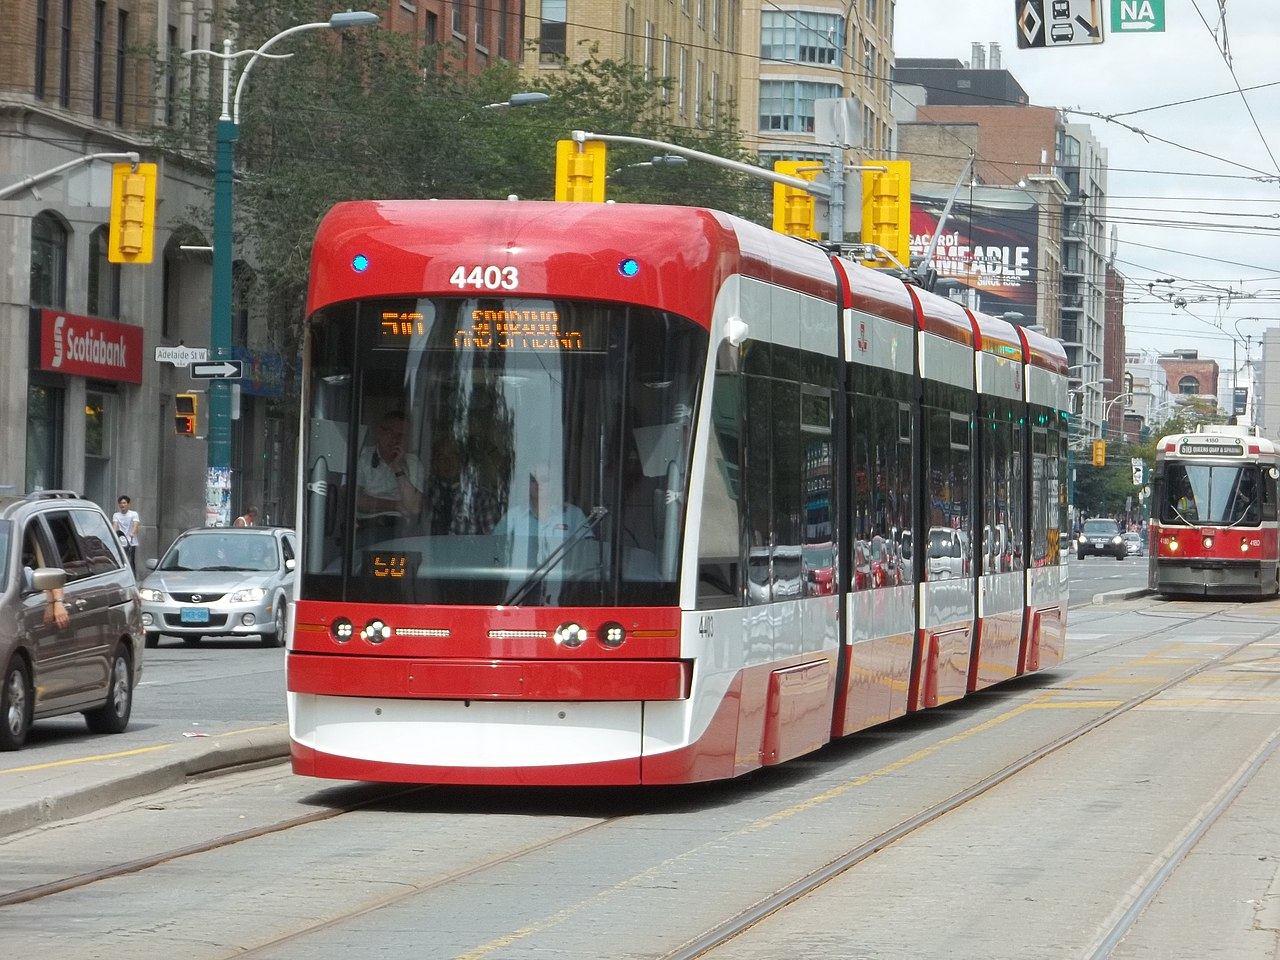
\includegraphics[width=1\linewidth]{images/spadina_streetcar.jpg}
			\end{figure}
			
		\end{column}
		
	\end{columns}
\end{frame}





\begin{frame}
	
	\textbf{Public Transit Benefits}: Efficiency
	
	\begin{figure}
		\centering
		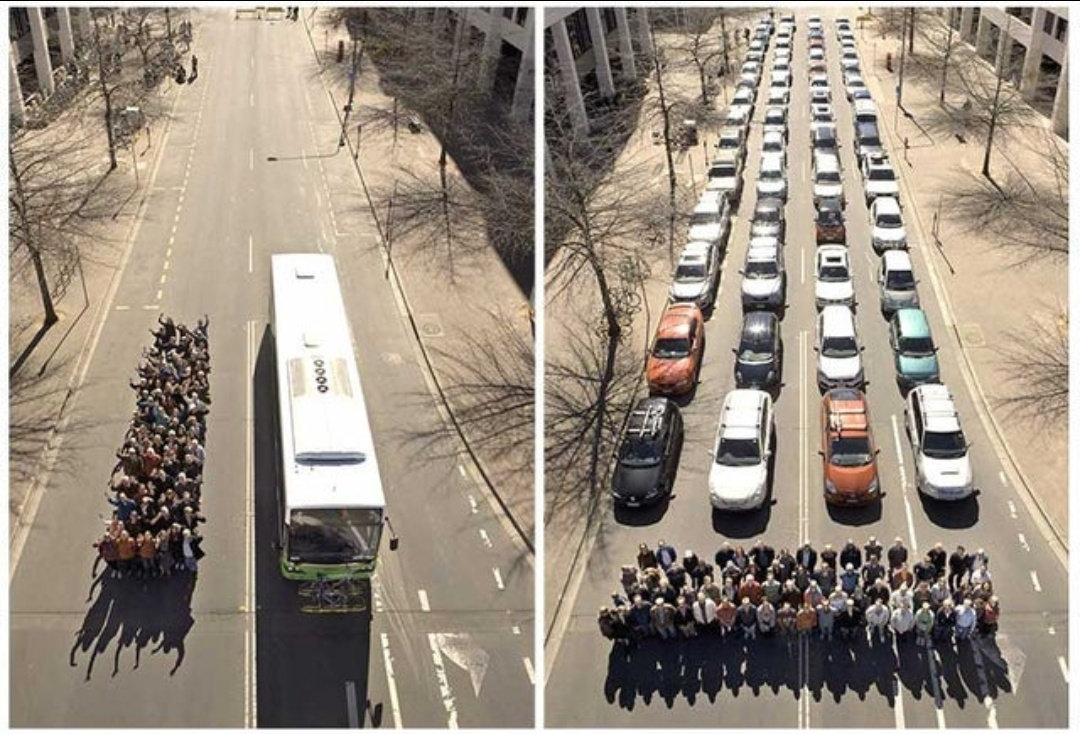
\includegraphics[width=0.8\linewidth]{images/transit_vs_car.jpg}
	\end{figure}

	\tiny\url{https://www.reddit.com/r/Damnthatsinteresting/comments/daugu5/public_transport_vs_private_transport/}
	
\end{frame}




\begin{frame}

	\textbf{What makes transit useful?} Seven demands of public transit:
	
	\vspace{2mm}
	
	\small
	\begin{enumerate}
		\item It takes me \textit{where} I want to go
		\item It takes me \textit{when} I want to go
		\item It is a good use of my \textit{time}
		\item It is a good use of my \textit{money}
		\item It \textit{respects} me in the level of safety, comfort, and amenity it provides
		\item I can \textit{trust} it
		\item It gives me \textit{freedom} to change my plans
	\end{enumerate}

	\vspace{2mm}
	
	Walker (2011)

\end{frame}


\begin{frame}
	
	
	
	\begin{columns}
		\begin{column}{0.5\textwidth}
			
			Components of a public transit system:
			
			\begin{itemize}
				\item \textbf{Network} - the combination of all connecting routes and stops
				
				\item \textbf{Routes} - connections between stops, usually fixed
				
				\item \textbf{Vehicles} - that traverse routes on set schedules
				
				\item \textbf{Stops} - where people access and exit the network, or transfer between routes
				
			\end{itemize}
			
			
		\end{column}
		
		\begin{column}{0.5\textwidth}
			\begin{figure}
				\centering
				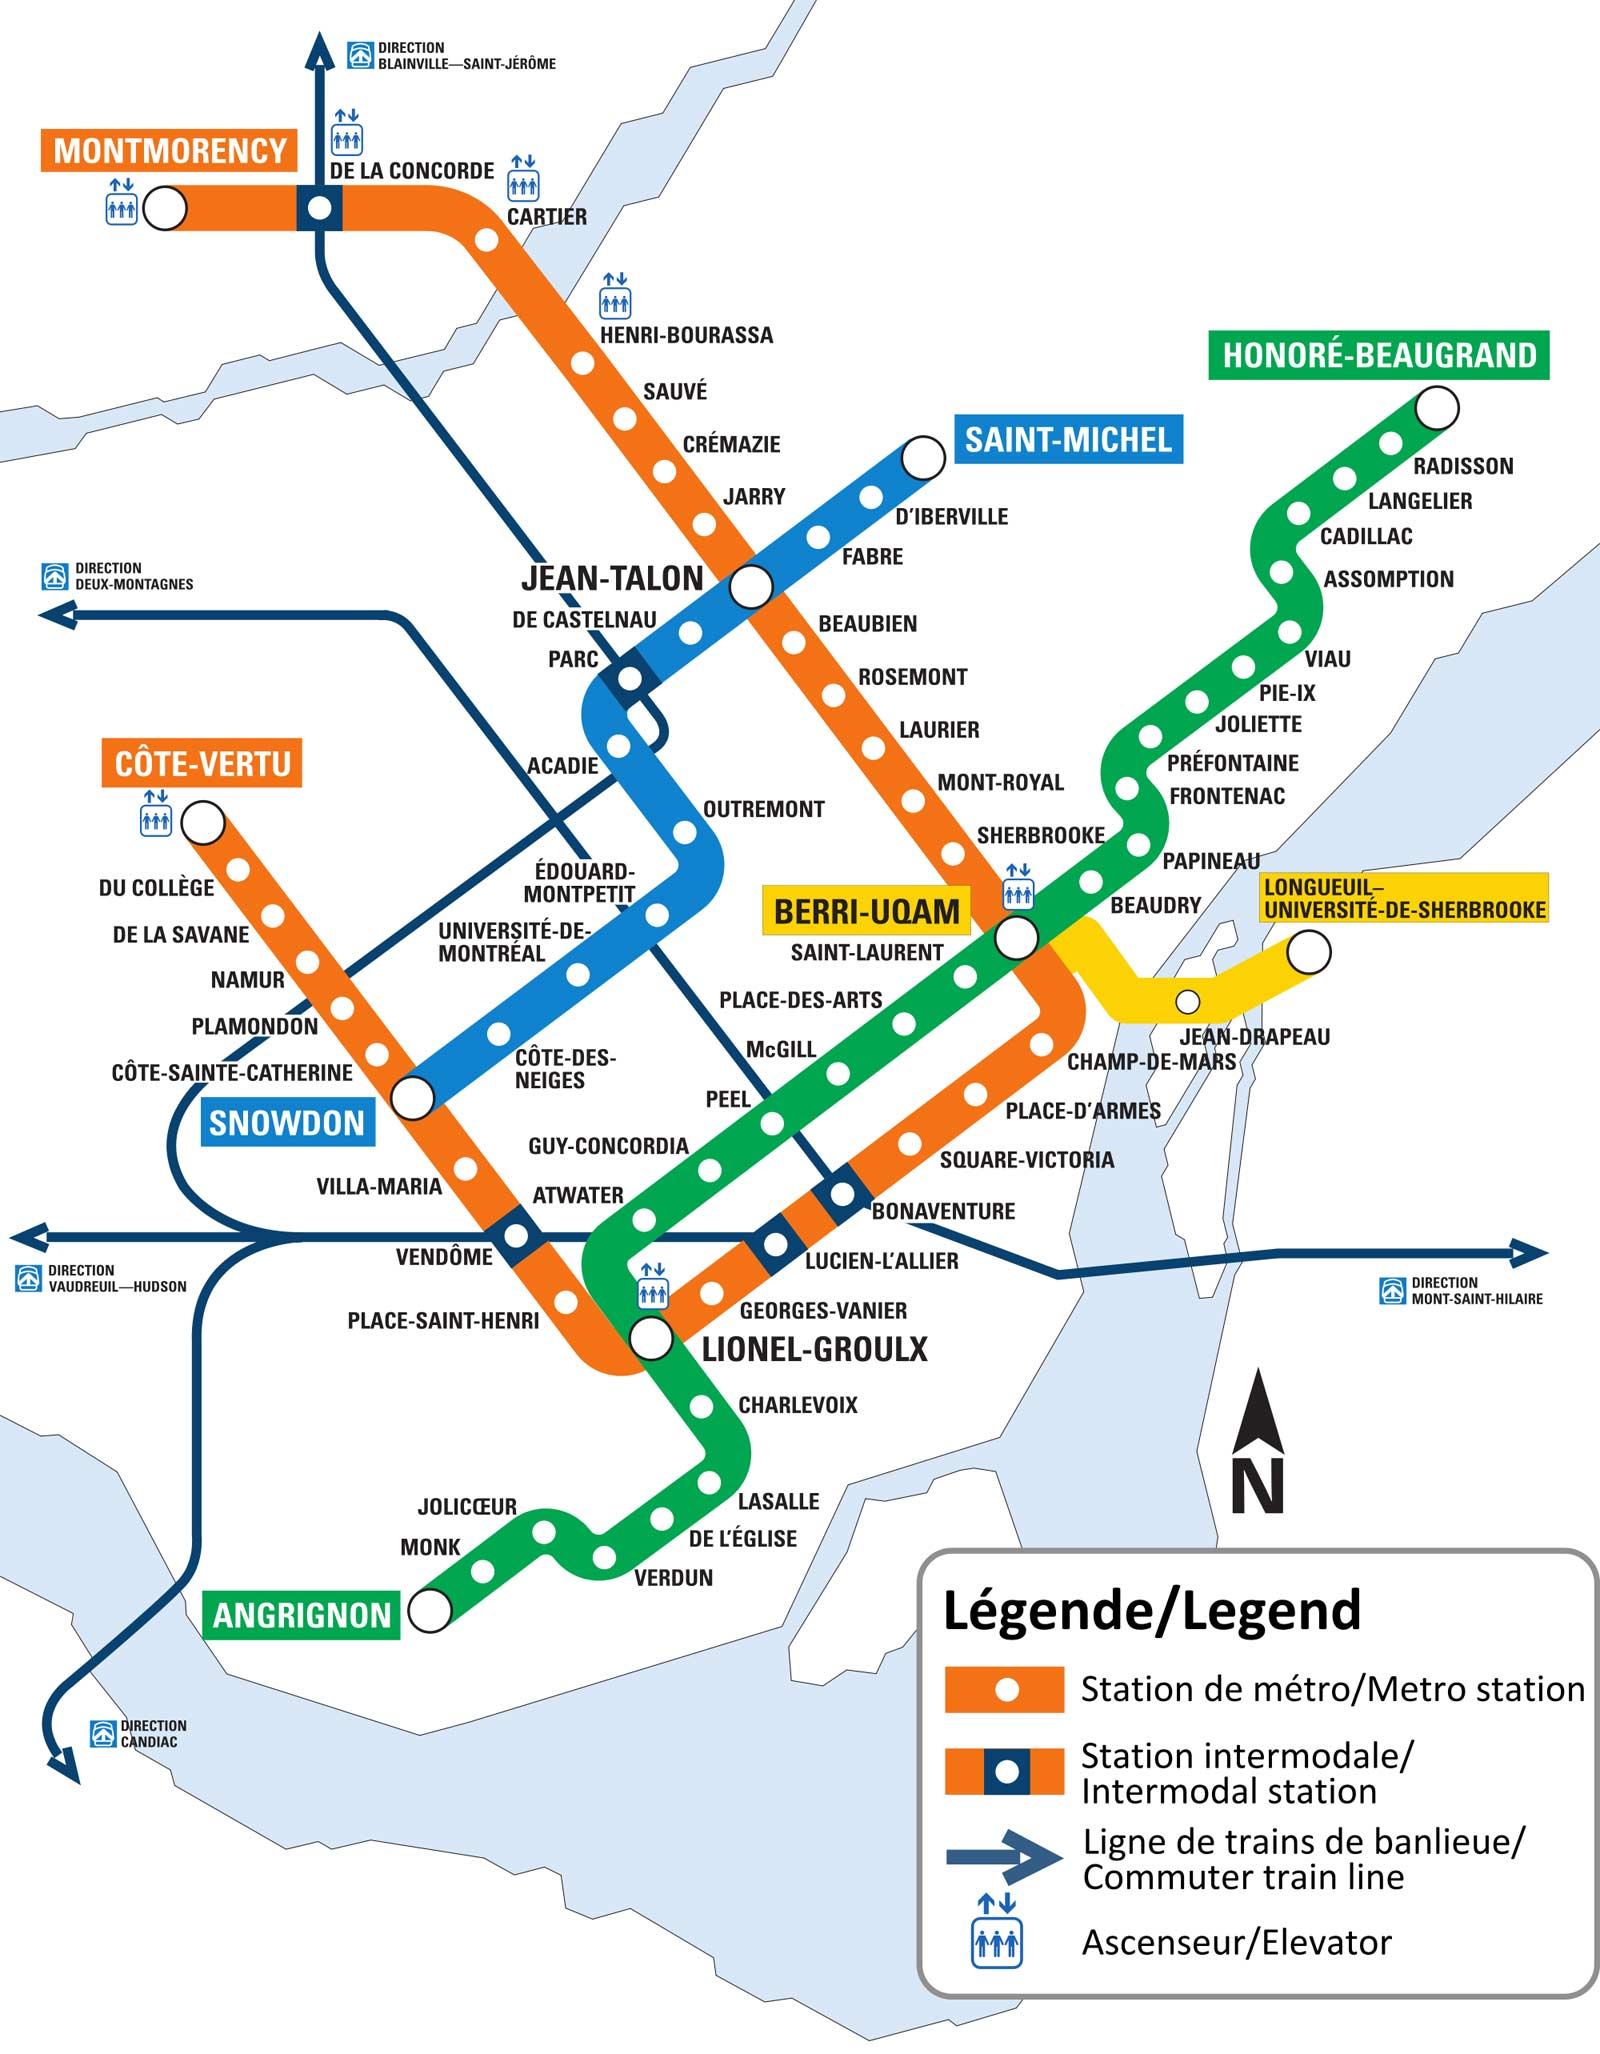
\includegraphics[width=1\linewidth]{images/montreal-metro-map.jpg}
			\end{figure}
			
		\end{column}
		
	\end{columns}
	
\end{frame}




\begin{frame}
	
	Types of transit network layouts: \textbf{Radial}
	
	\begin{figure}
		\centering
		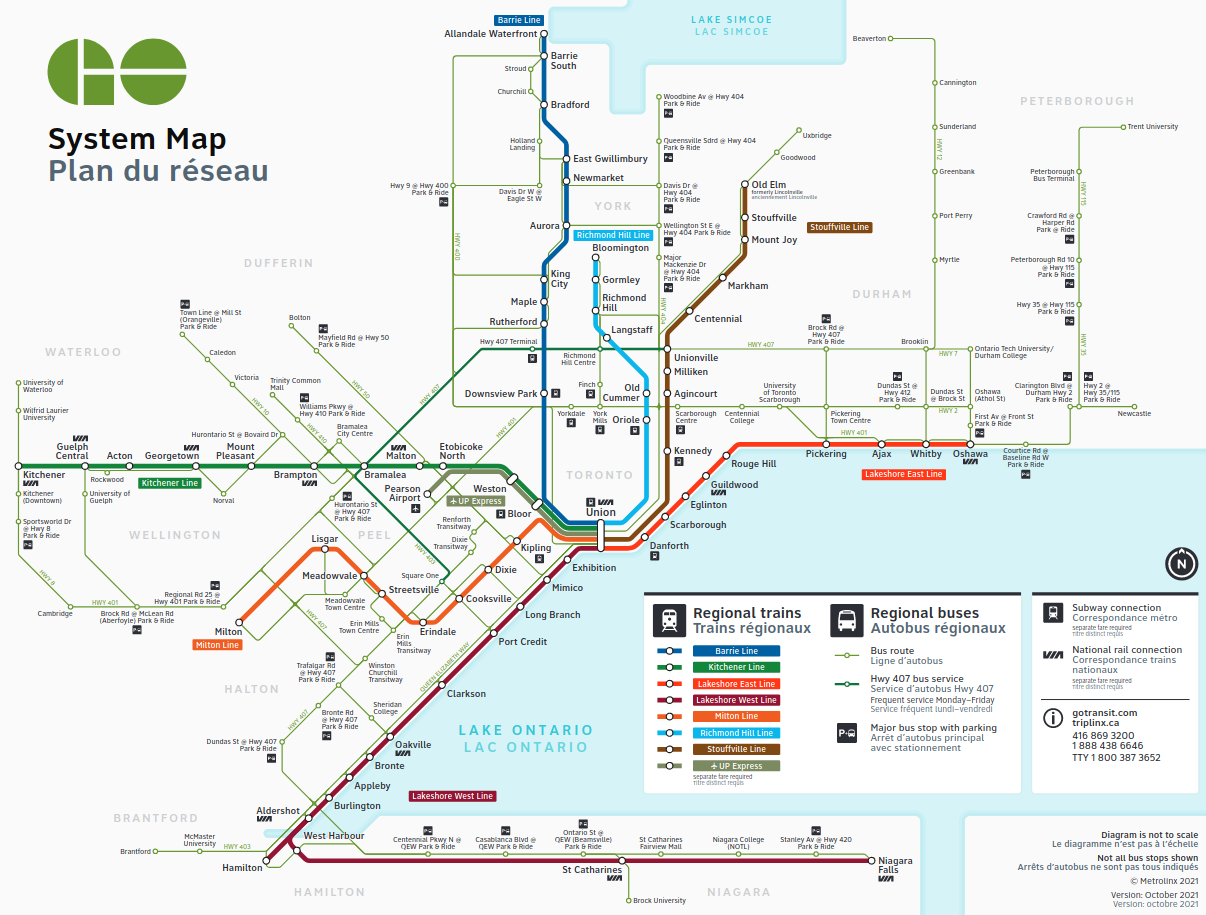
\includegraphics[width=0.7\linewidth]{images/go_map.png}
	\end{figure}

	\tiny\url{https://www.gotransit.com/en/trip-planning/system-and-route-map}
	
\end{frame}



\begin{frame}
	
	Types of transit network layouts: \textbf{Grid}
	
	\begin{figure}
		\centering
		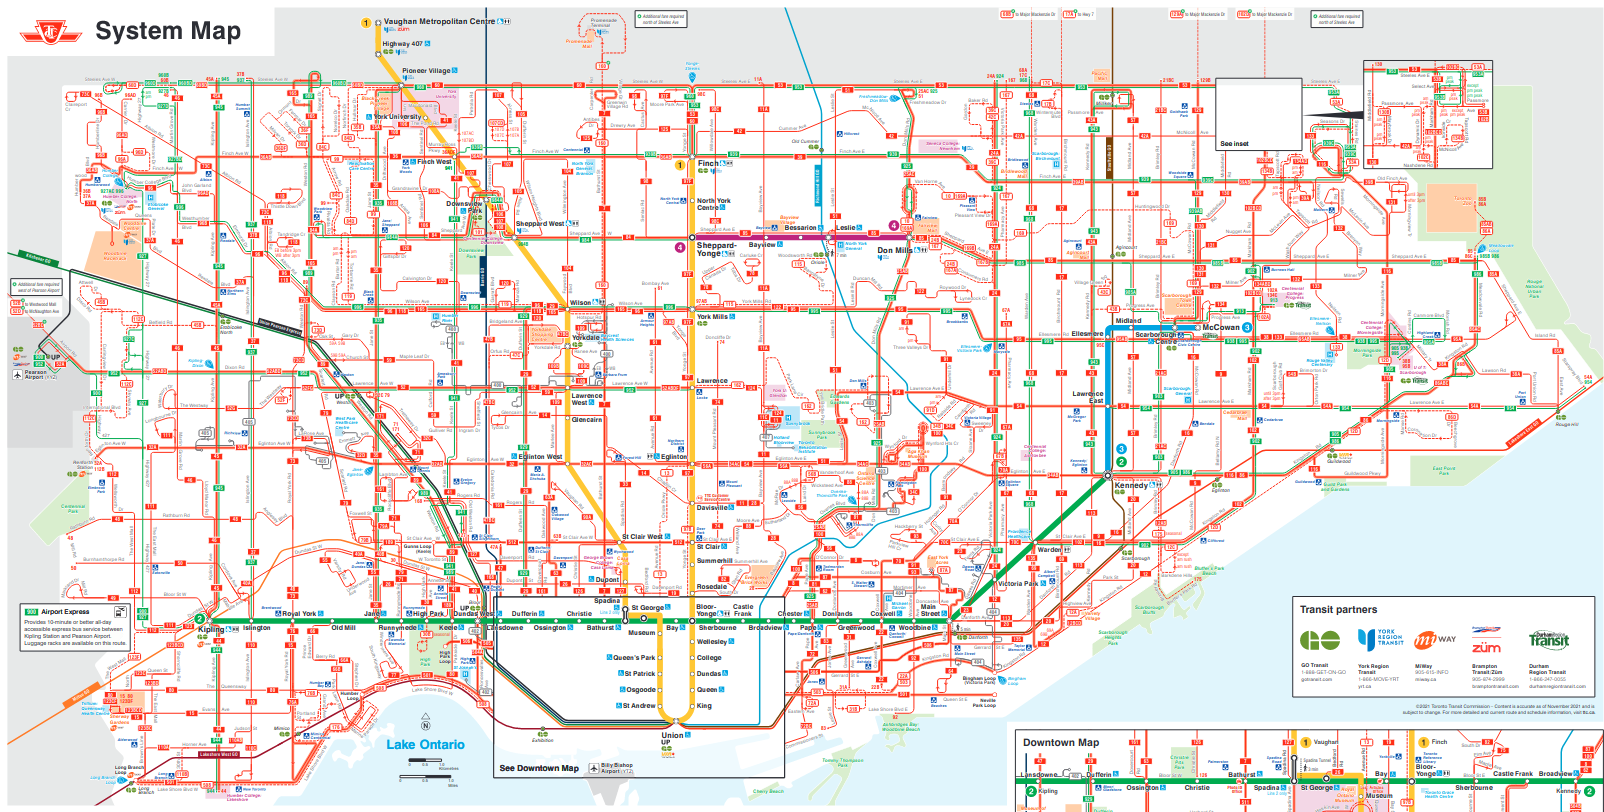
\includegraphics[width=1\linewidth]{images/ttc-map.png}
	\end{figure}

	\tiny\url{https://www.ttc.ca/routes-and-schedules/}
	
\end{frame}


\begin{frame}
	
	Types of transit network layouts: \textbf{Circle-Radial}
	
	\begin{figure}
		\centering
		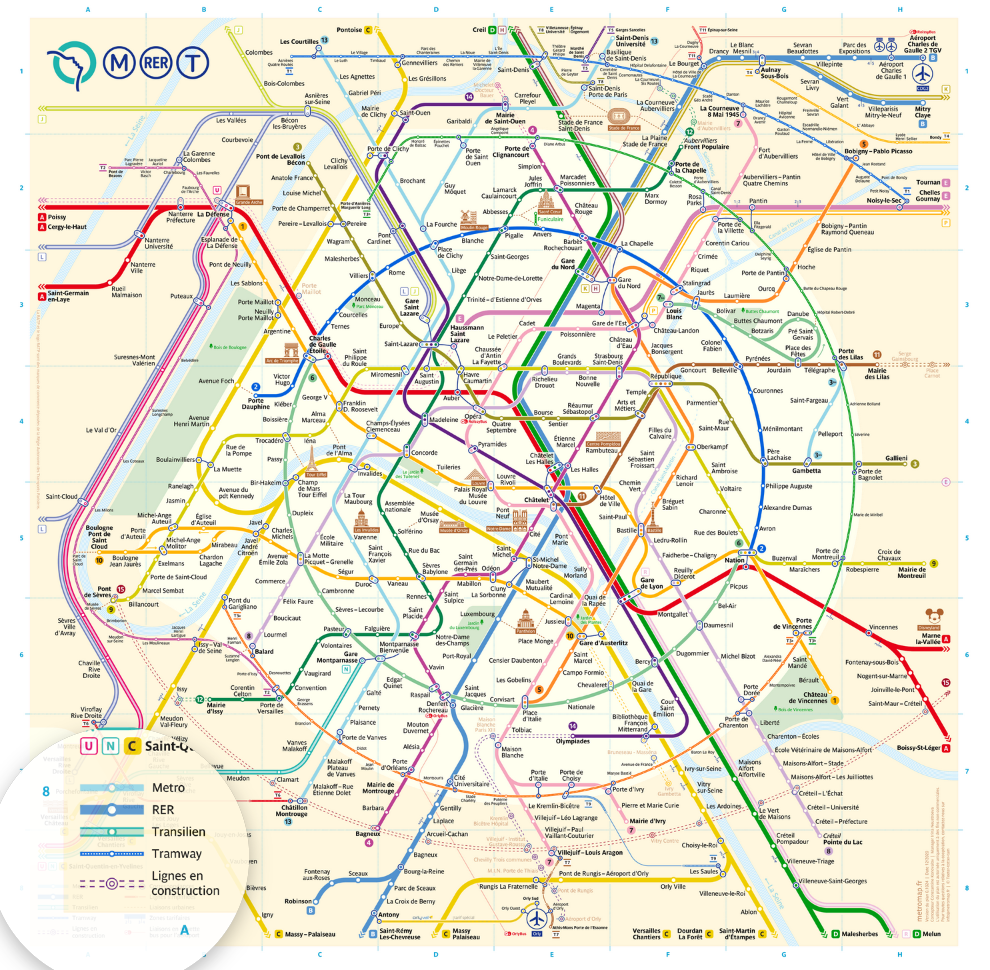
\includegraphics[width=0.6\linewidth]{images/paris_metro.png}
	\end{figure}
	
	
	\tiny \url{https://metromap.fr/en}
\end{frame}




\begin{frame}
	
	Types of transit network layouts: 
	
	\begin{figure}
		\centering
		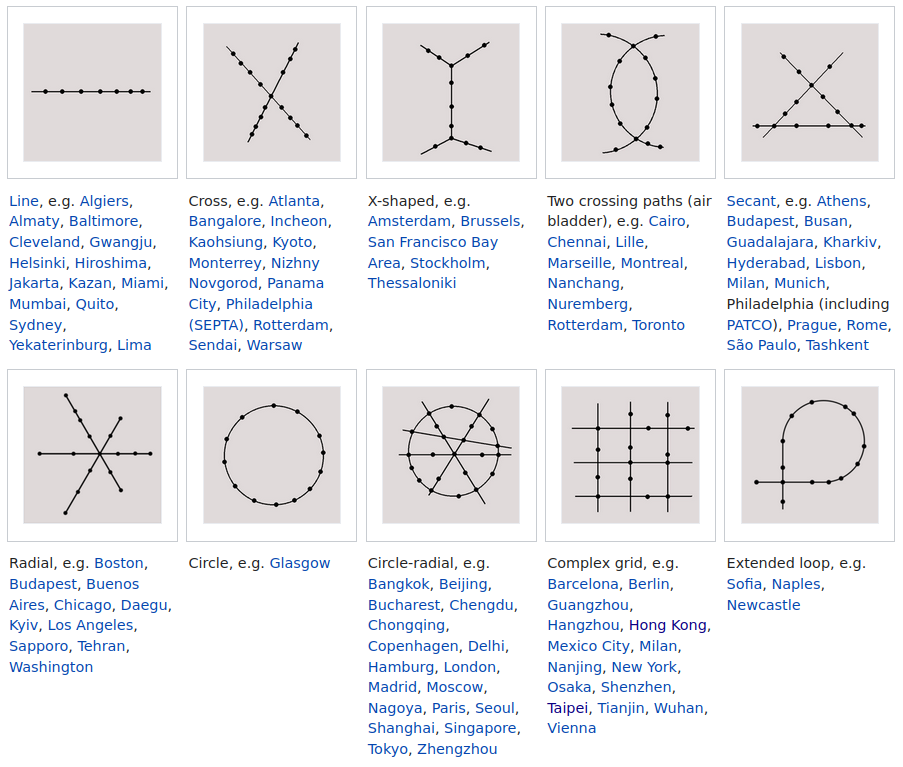
\includegraphics[width=0.6\linewidth]{images/network_designs.png}
	\end{figure}
	
	
	\tiny \url{https://en.wikipedia.org/wiki/Rapid_transit}
\end{frame}






\begin{frame}
	
	
	
	\begin{columns}
		\begin{column}{0.5\textwidth}
			
			\textbf{Route Characteristics:	}
			
			\vspace{2mm}
			\begin{itemize}
				\item Technology
				\item Level of separation from other transport
				\item Capacity
				\item Comfort/Safety
				\item Frequency
				\item Stop Spacing
				\item Reliability
				\item Network hierarchy
			\end{itemize}
			
			
		\end{column}
		
		\begin{column}{0.5\textwidth}
			\begin{figure}
				\centering
				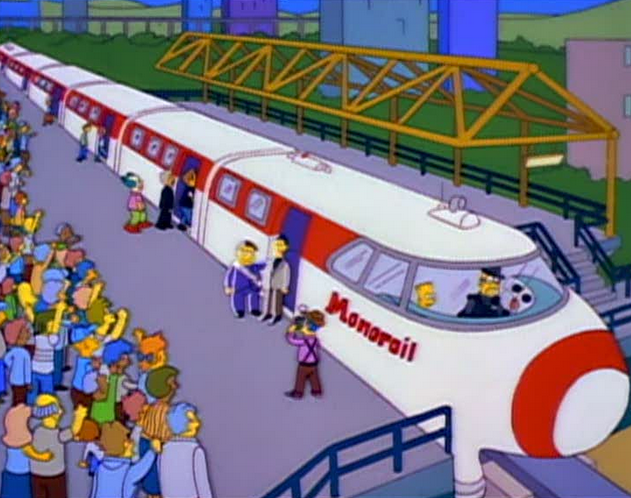
\includegraphics[width=0.98\linewidth]{images/monorail.png}
			\end{figure}
			
		\end{column}
		
	\end{columns}
	

	
\end{frame}





\begin{frame}
	
	\textbf{Routes} - Technology 
	
	\begin{figure}
		\centering
		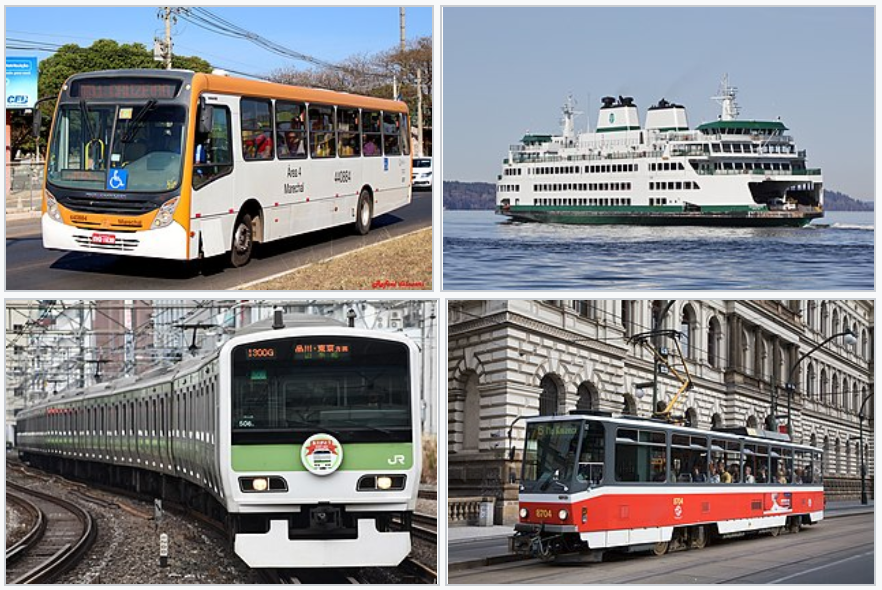
\includegraphics[width=0.76\linewidth]{images/wiki_transit.png}
	\end{figure}
	
	\tiny \url{https://en.wikipedia.org/wiki/Public_transport}
	
\end{frame}






\begin{frame}
	\begin{columns}
		\begin{column}{0.6\textwidth}
			
			\textbf{Routes} - Level of separation from other transport
			
			
			\begin{enumerate}
				
				\item Completely separated (can be above, below, or at ground-level)
				\begin{itemize}
					\item e.g. TTC Subway Lines
				\end{itemize}
				
				\item Separated from other traffic, but with at-grade crossing
				\begin{itemize}
					\item e.g. Spadina Streetcar, Eglinton LRT, Highway 7 BRT
				\end{itemize}
				
				\item Shared with traffic
				\begin{itemize}
					\item e.g. Most TTC bus and streetcar routes
				\end{itemize}
				
			\end{enumerate}
			
		\end{column}
		
		\begin{column}{0.4\textwidth}
			\begin{figure}
				\centering
				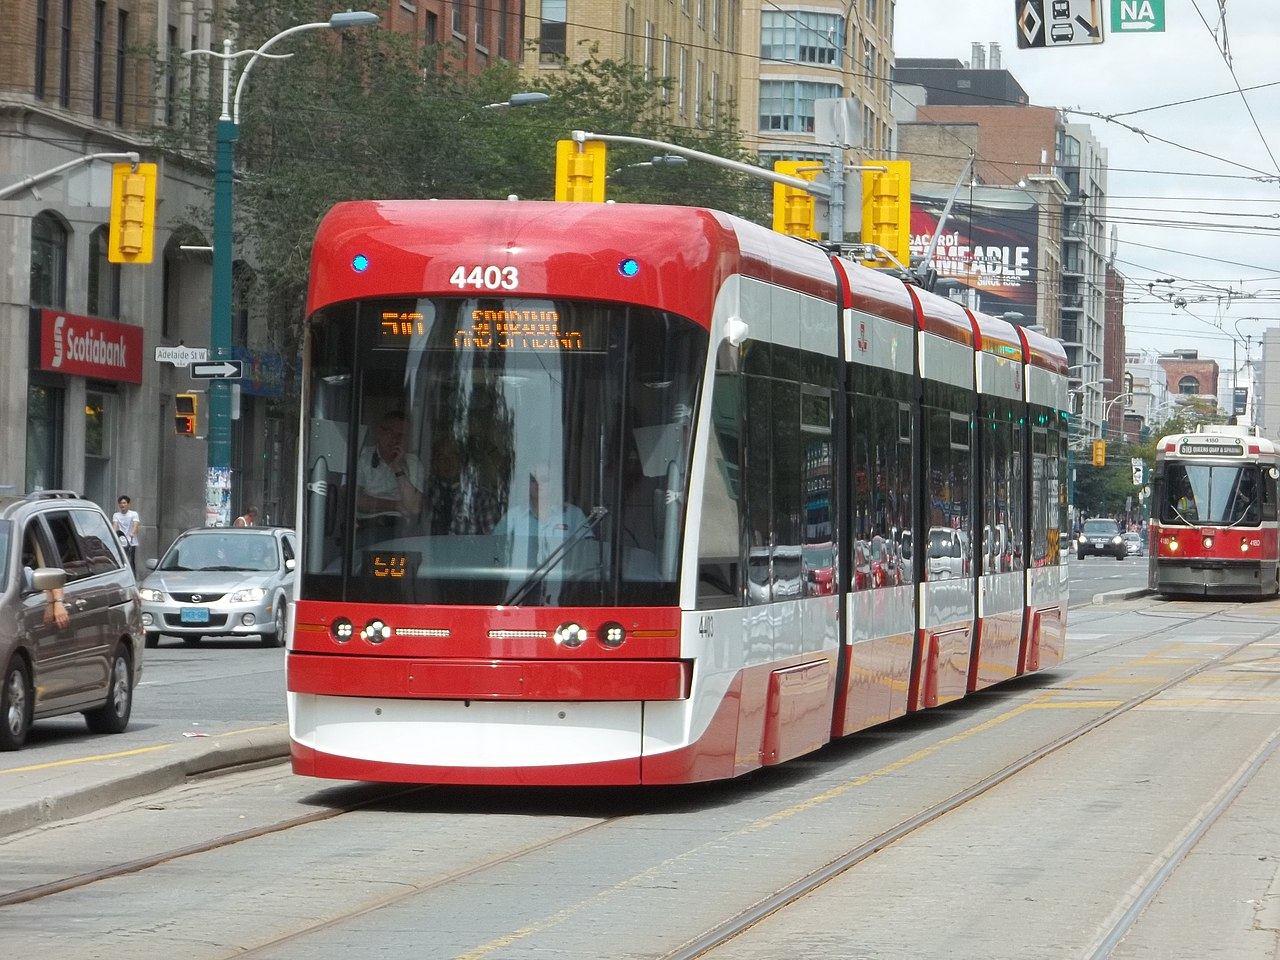
\includegraphics[width=1\linewidth]{images/spadina_streetcar.jpg}
			\end{figure}
			
		\end{column}
		
	\end{columns}
\end{frame}






\begin{frame}
	
	\textbf{Routes} - Level of separation from other transport
	
	
	\begin{itemize}
		
		\item[1.] Completely separated (can be above, below, or at ground-level)
		
		\begin{itemize}
			\item many names, e.g. Rapid Transit, Metro, Underground, Heavy Rail, etc.
			\item Run in exclusive Rights Of Way (ROW)
		\end{itemize}
		
	\end{itemize}

	\begin{figure}
		\centering
		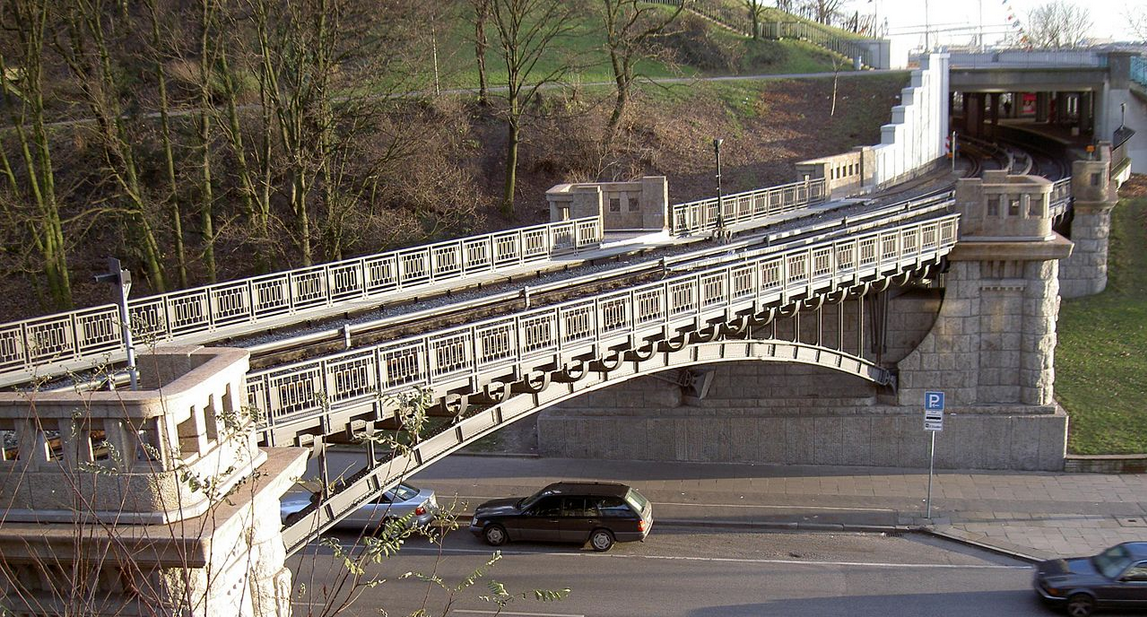
\includegraphics[width=0.7\linewidth]{images/hamburg.png}
	\end{figure}

	
	
\end{frame}




\begin{frame}
	
	\textbf{Routes} - Level of separation from other transport
	
	
	\begin{itemize}
		
		\item[2.] Separated from other traffic, but with at-grade crossing
		
		\begin{itemize}
			\item LRT (Light Rail Transit)
			\item BRT (Bus Rapid Transit)
		\end{itemize}
		
	\end{itemize}
	
	\begin{figure}
		\centering
		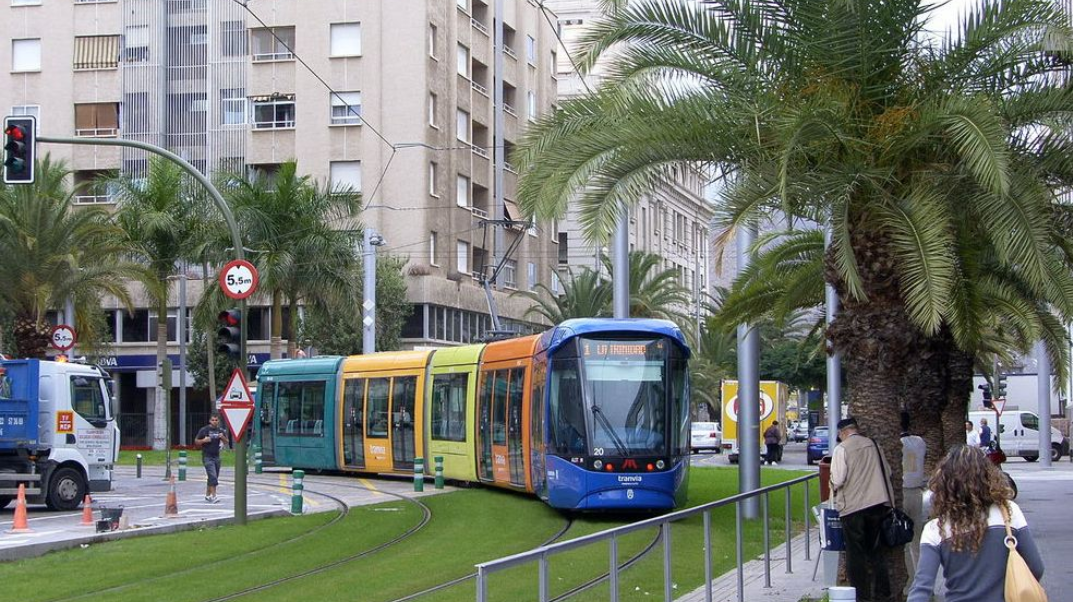
\includegraphics[width=0.7\linewidth]{images/lrt_spain.png}
	\end{figure}
	
	\tiny\url{https://en.wikipedia.org/wiki/Light_rail}
	
	
\end{frame}











\begin{frame}
	
	\textbf{Routes} - Level of separation from other transport
	
	
	\begin{itemize}
		
		\item[2.] Separated from other traffic, but with at-grade crossing
		
		\begin{itemize}
			\item LRT (Light Rail Transit)
			\item BRT (Bus Rapid Transit)
		\end{itemize}
		
	\end{itemize}
	
	\begin{figure}
		\centering
		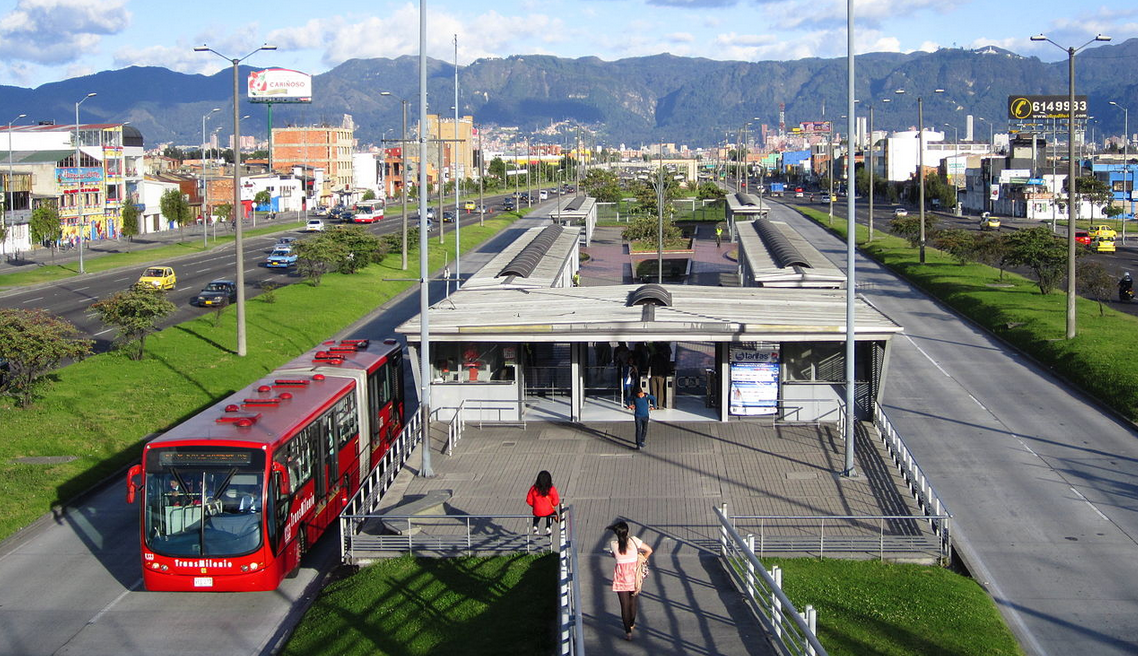
\includegraphics[width=0.7\linewidth]{images/transmilenio.png}
	\end{figure}
	
	\tiny\url{https://en.wikipedia.org/wiki/TransMilenio}
	
	
\end{frame}





\begin{frame}
	
	\textbf{Routes} - Level of separation from other transport
	
	
	\begin{itemize}
		
		\item[3.] Shared with traffic
		
		
	\end{itemize}
	
	\begin{figure}
		\centering
		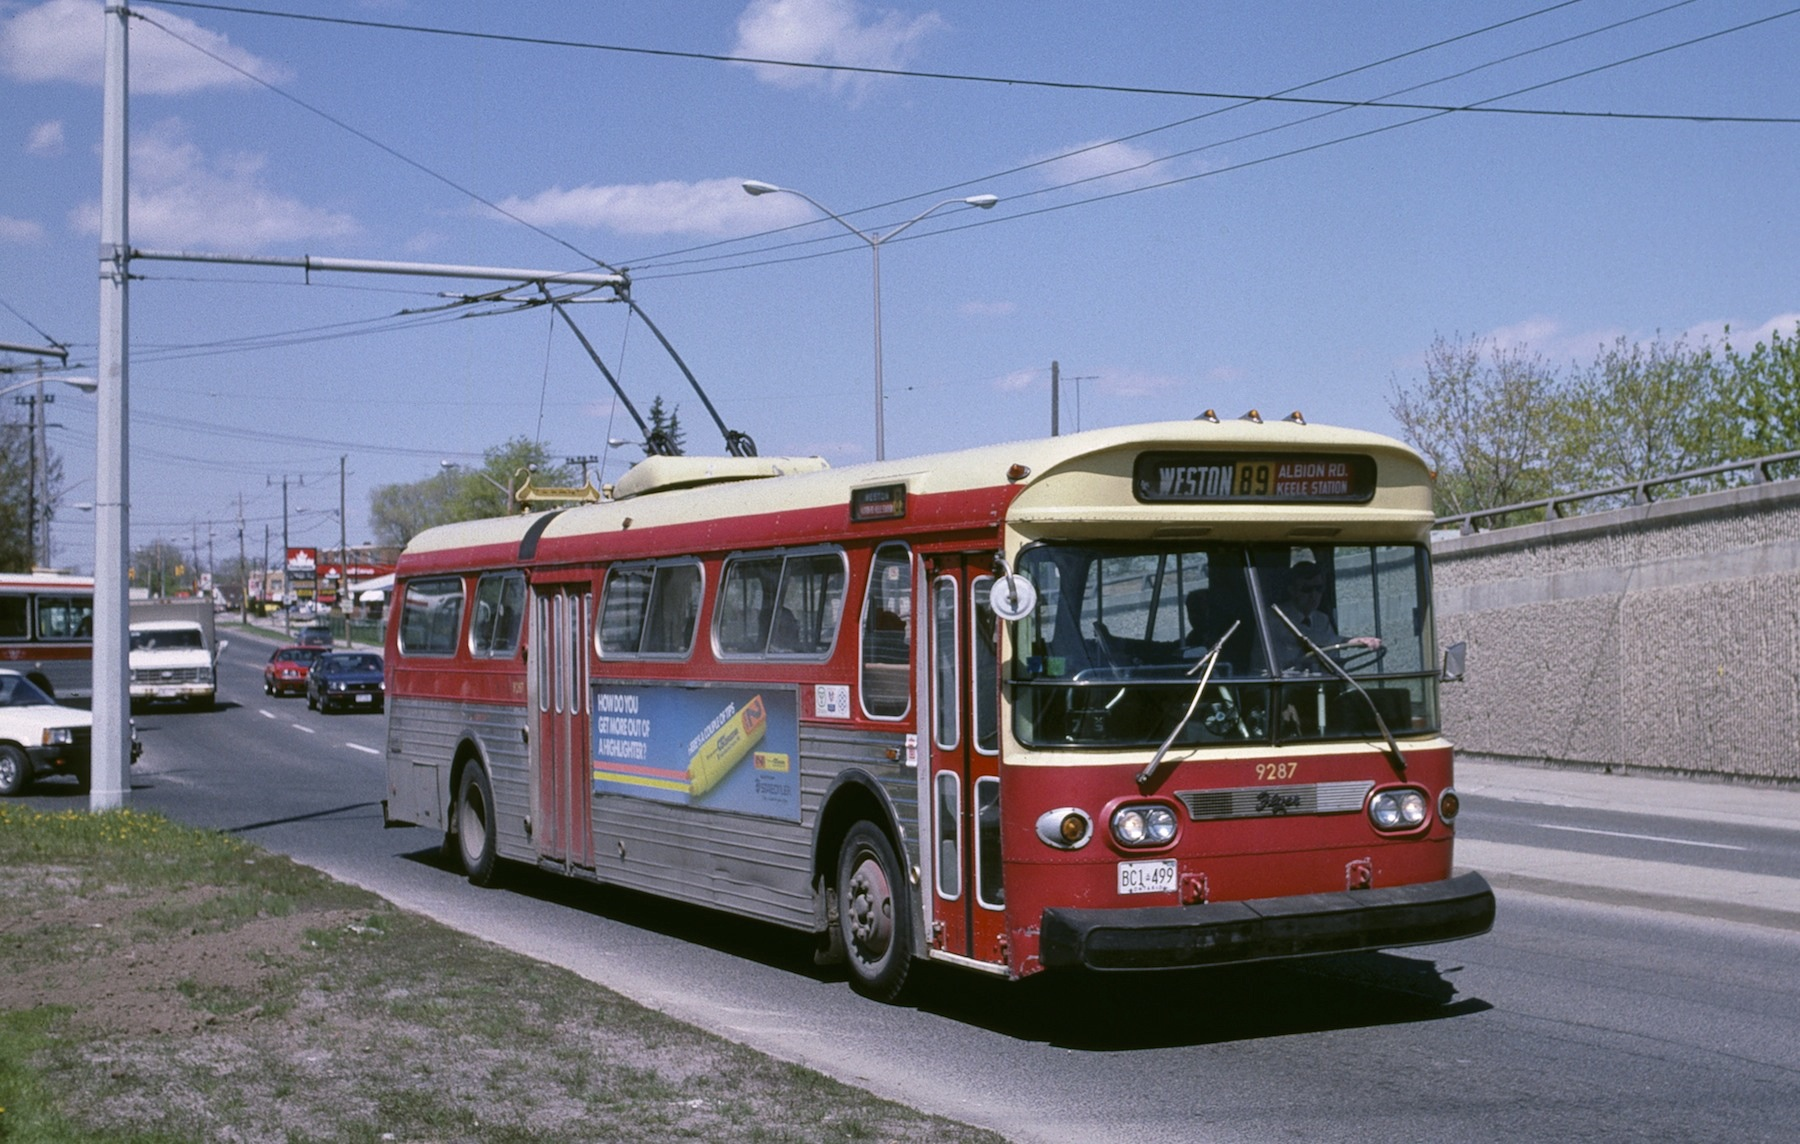
\includegraphics[width=0.77\linewidth]{images/trolleybus.jpg}
	\end{figure}
	
	\tiny\url{https://en.wikipedia.org/wiki/Bus}
	
	
\end{frame}






\begin{frame}
	
	\textbf{Routes} - Capacity
	
	\vspace{2mm}
	
	Can be measured per vehicle, or per route in a given time (e.g. an hour)
	
	\begin{columns}
		\begin{column}{0.5\textwidth}
			
			\begin{figure}
				\centering
				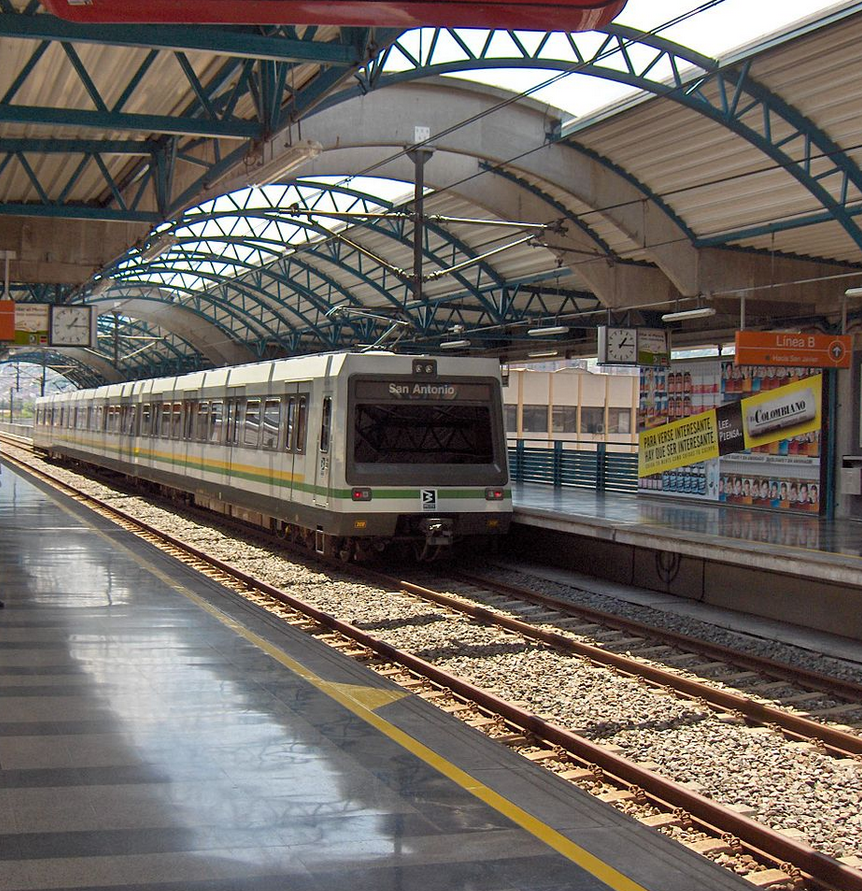
\includegraphics[width=0.9\linewidth]{images/metro_medellin.png}
			\end{figure}
			
			
		\end{column}
		
		\begin{column}{0.5\textwidth}
			\begin{figure}
				\centering
				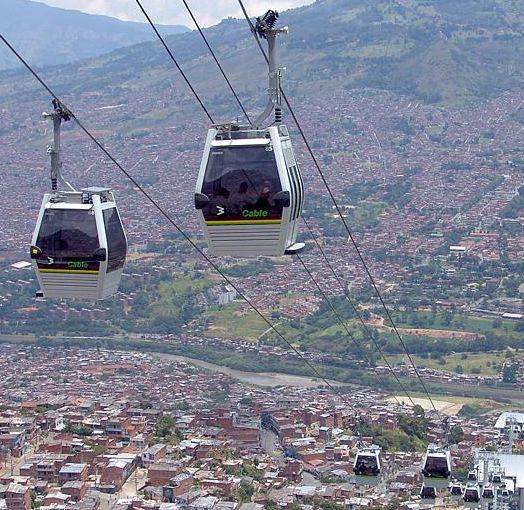
\includegraphics[width=1\linewidth]{images/metrocable.jpg}
			\end{figure}
			
		\end{column}
		
	\end{columns}
	
	\tiny\url{https://en.wikipedia.org/wiki/Medellin_Metro}
	
\end{frame}





\begin{frame}
	
	\textbf{Routes} - Comfort \& Safety
	
	\vspace{2mm}
	
	Some components can be measured like crowding, but many are subjective 
	
	 \begin{figure}
	 	\centering
	 	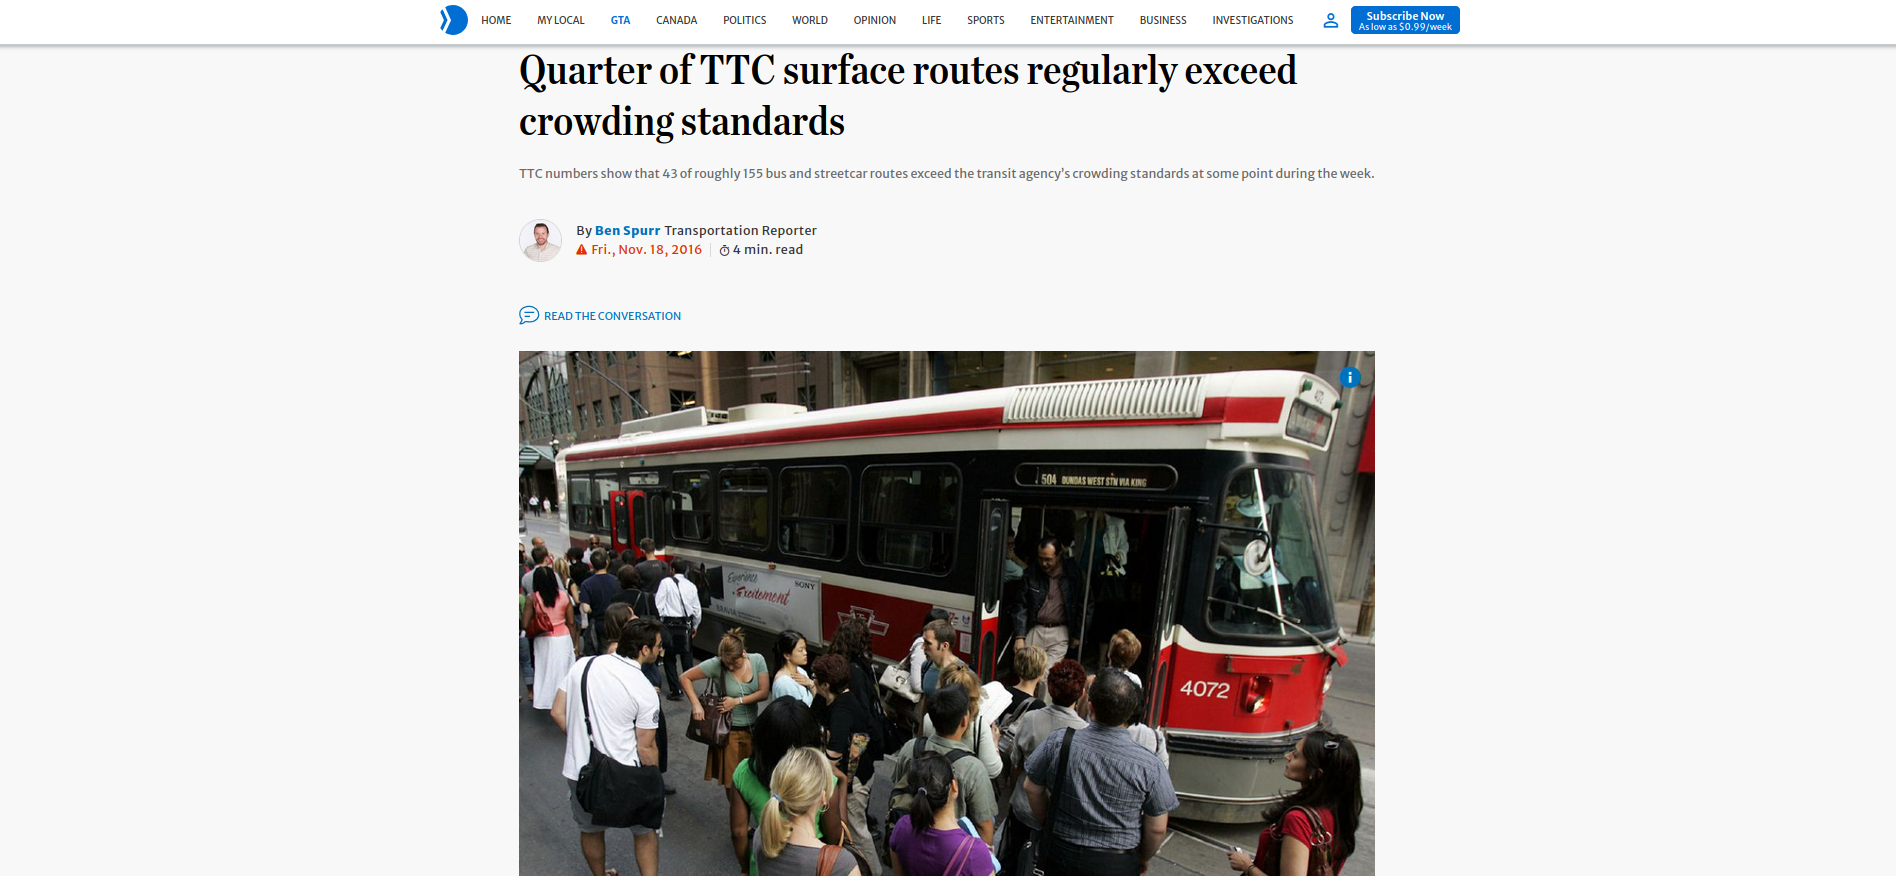
\includegraphics[width=1\linewidth]{images/crowding.png}
	 \end{figure}
	
	
	
	
\end{frame}





\begin{frame}
	
	
	
	
	\begin{columns}
		\begin{column}{0.5\textwidth}
			
			\textbf{Routes} - Frequency
			
			\vspace{4mm}
			
			In transit planning \& operations, frequency is often measured by a routes scheduled \textbf{headway}, the time between vehicles
			
			\vspace{4mm}
			
			"Frequency is freedom" - Walker
			
			
		\end{column}
		
		\begin{column}{0.5\textwidth}
			\small example of a TTC stop schedule (501)
			\begin{figure}
				\centering
				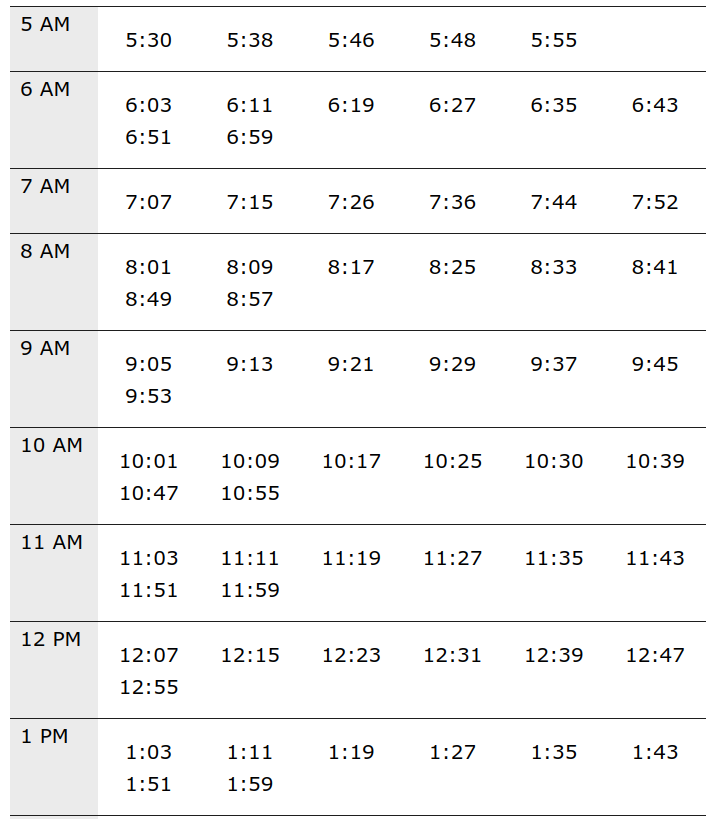
\includegraphics[width=1\linewidth]{images/ttc_schedule_eg.png}
			\end{figure}
			
		\end{column}
		
	\end{columns}
	
\end{frame}


\begin{frame}
	
	\textbf{Routes} - Frequency
	
	\vspace{2mm}
	
	e.g. bus that comes every 30 minutes, until midnight, 7 days a week:
	
	\begin{figure}
		\centering
		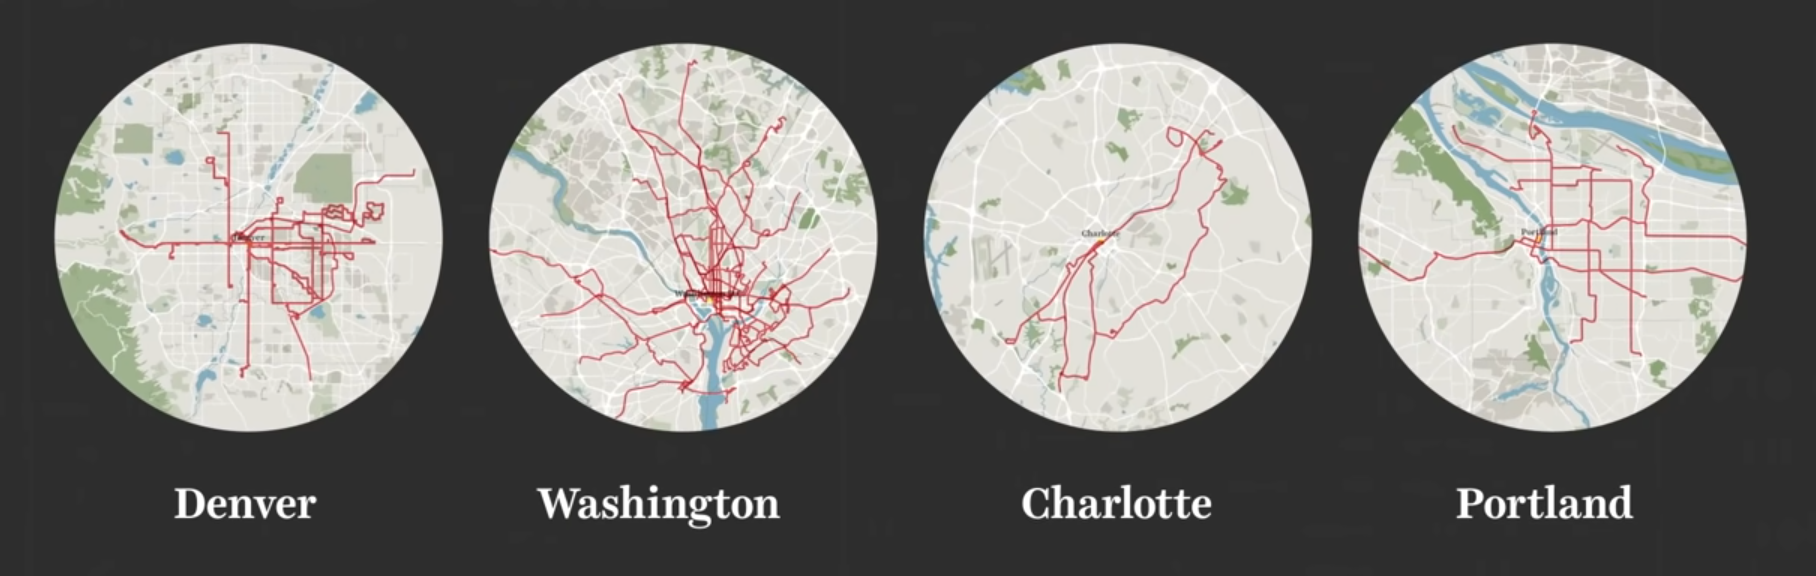
\includegraphics[width=1\linewidth]{images/frequency_usa.png}
	\end{figure}

	\tiny\url{https://www.youtube.com/watch?v=-ZDZtBRTyeI}
	
\end{frame}


\begin{frame}
	
	\textbf{Routes} - Frequency
	
	\begin{figure}
		\centering
		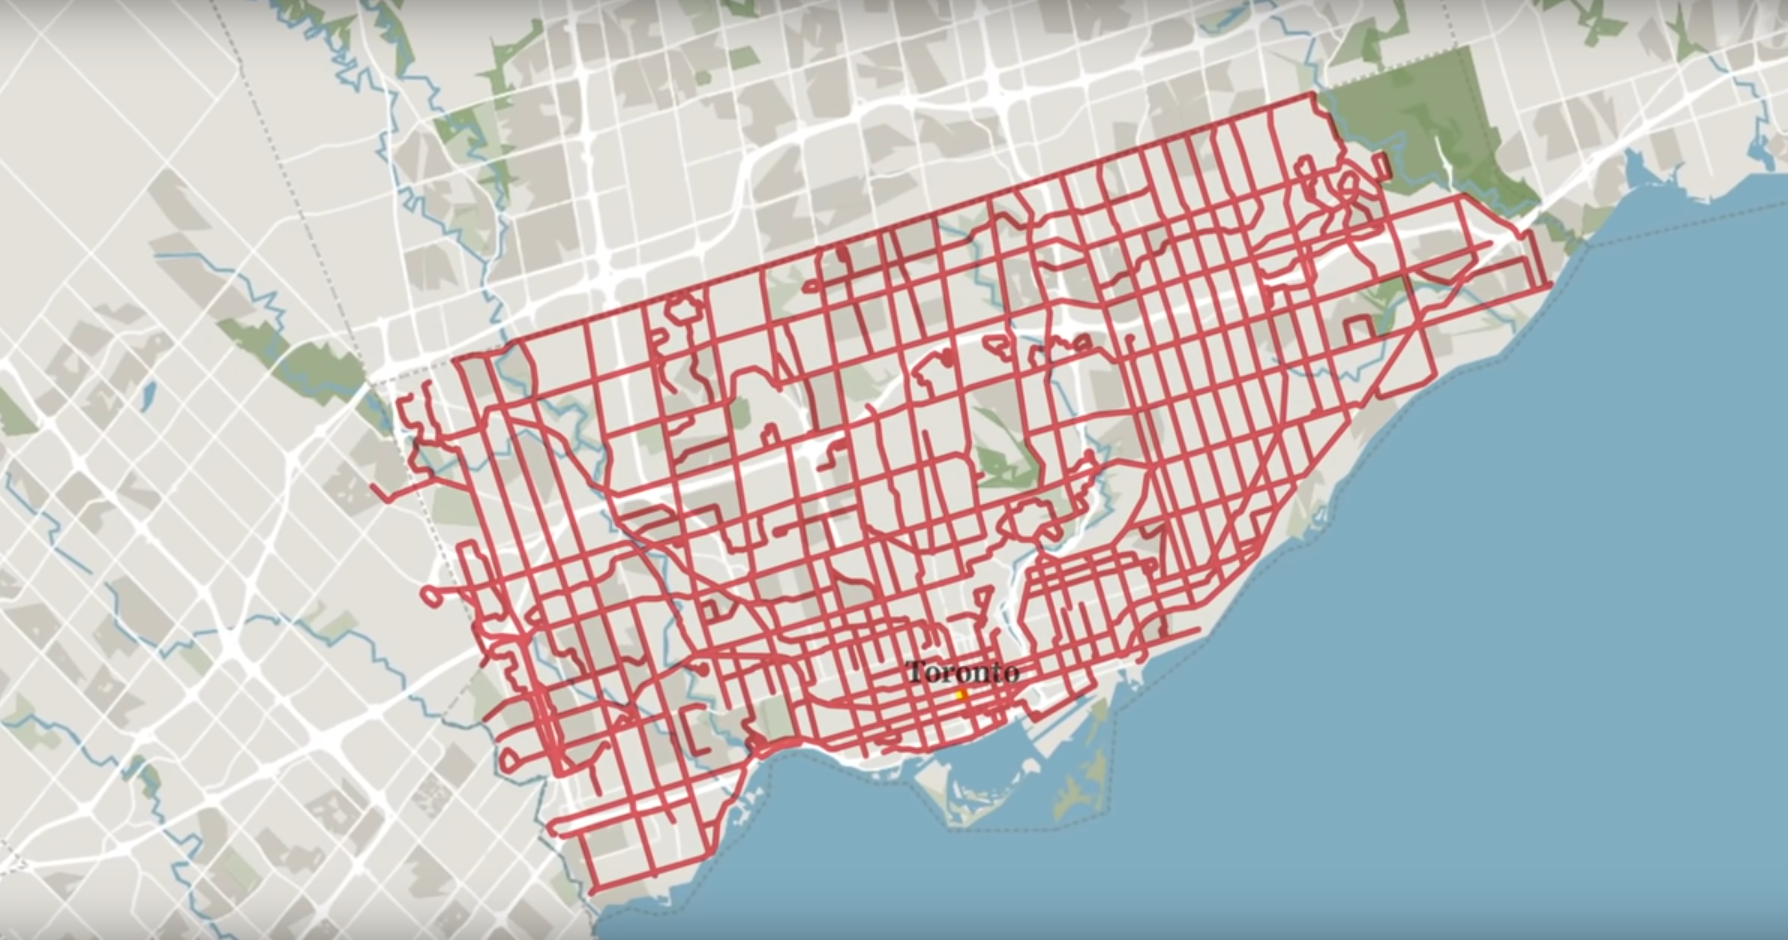
\includegraphics[width=1\linewidth]{images/toronto_frequency.png}
	\end{figure}

	\tiny\url{https://www.youtube.com/watch?v=-ZDZtBRTyeI}
	
\end{frame}



\begin{frame}
	
	\textbf{Routes} - Frequency
	
	\begin{figure}
		\centering
		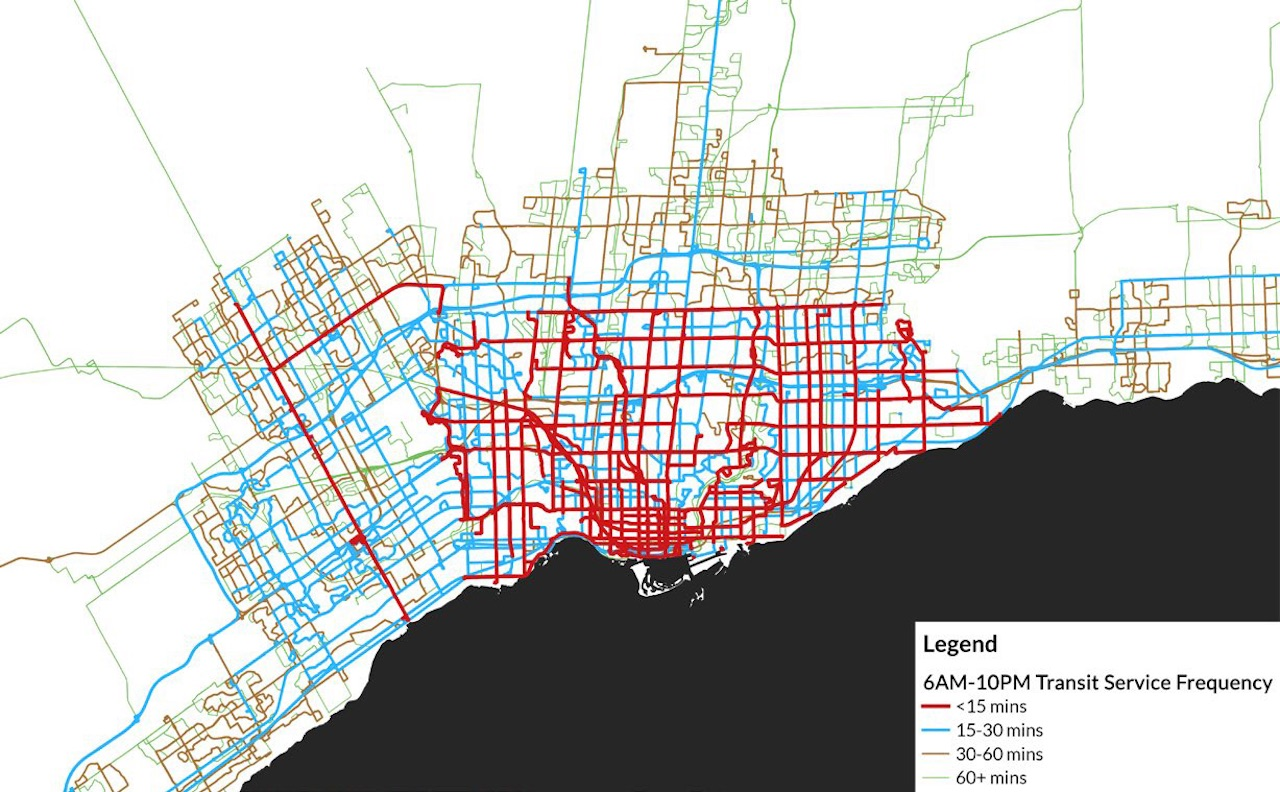
\includegraphics[width=0.8\linewidth]{images/gta_frequency.jpg}
	\end{figure}

	\tiny\url{https://urbantoronto.ca/news/2021/11/board-trade-urges-frequent-transit-service-across-region}
	
\end{frame}




\begin{frame}
	
	\textbf{Routes} - Stop Spacing
	
	\vspace{2mm}
	
	TTC Bus \& Streetcar routes have stops every 100m-300m
		
	\vspace{2mm}
	
	More stops means better local access, but reduced speeds and longer travel times because the vehicle needs to make more stops. i.e. a trade-off.
	
	\begin{figure}
		\centering
		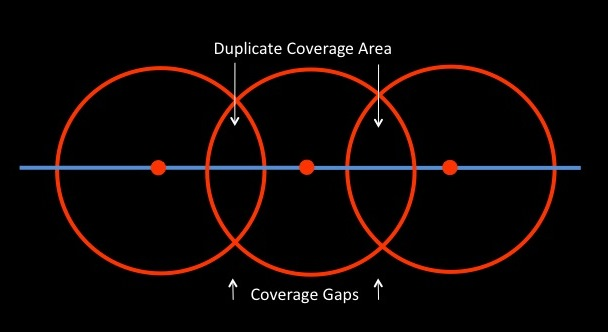
\includegraphics[width=0.6\linewidth]{images/stop_spacing.jpg}
	\end{figure}
	
	
	\tiny \url{https://humantransit.org/2010/11/san-francisco-a-rational-stop-spacing-plan.html}
	
\end{frame}



\begin{frame}
	
	\textbf{Routes} - Stop Spacing
	
	\vspace{2mm}
	
	Local access to a stop depends on urban form / street networks (more on this next week)
	
	\begin{columns}
		\begin{column}{0.5\textwidth}
			
			\begin{figure}
				\centering
				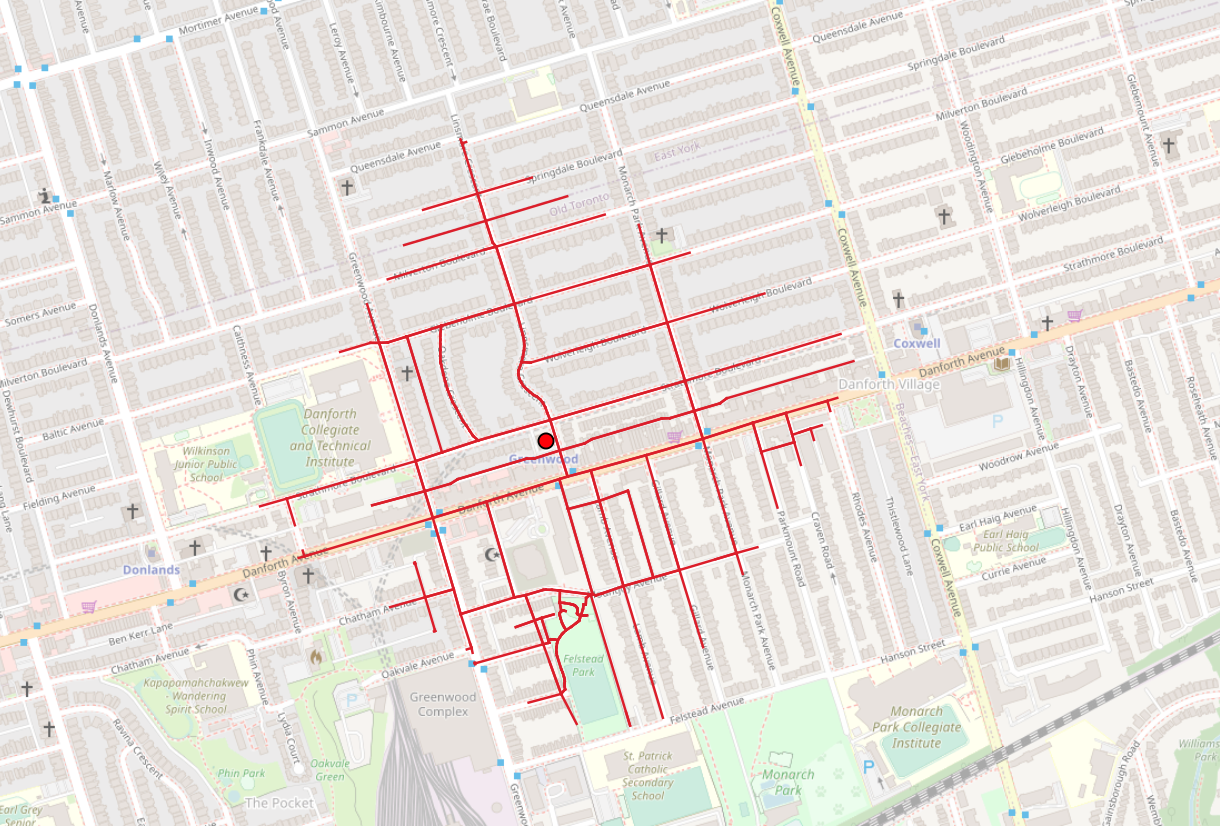
\includegraphics[width=1\linewidth]{images/greenwood.png}
			\end{figure}
			
			
		\end{column}
		
		\begin{column}{0.5\textwidth}
			\begin{figure}
				\centering
				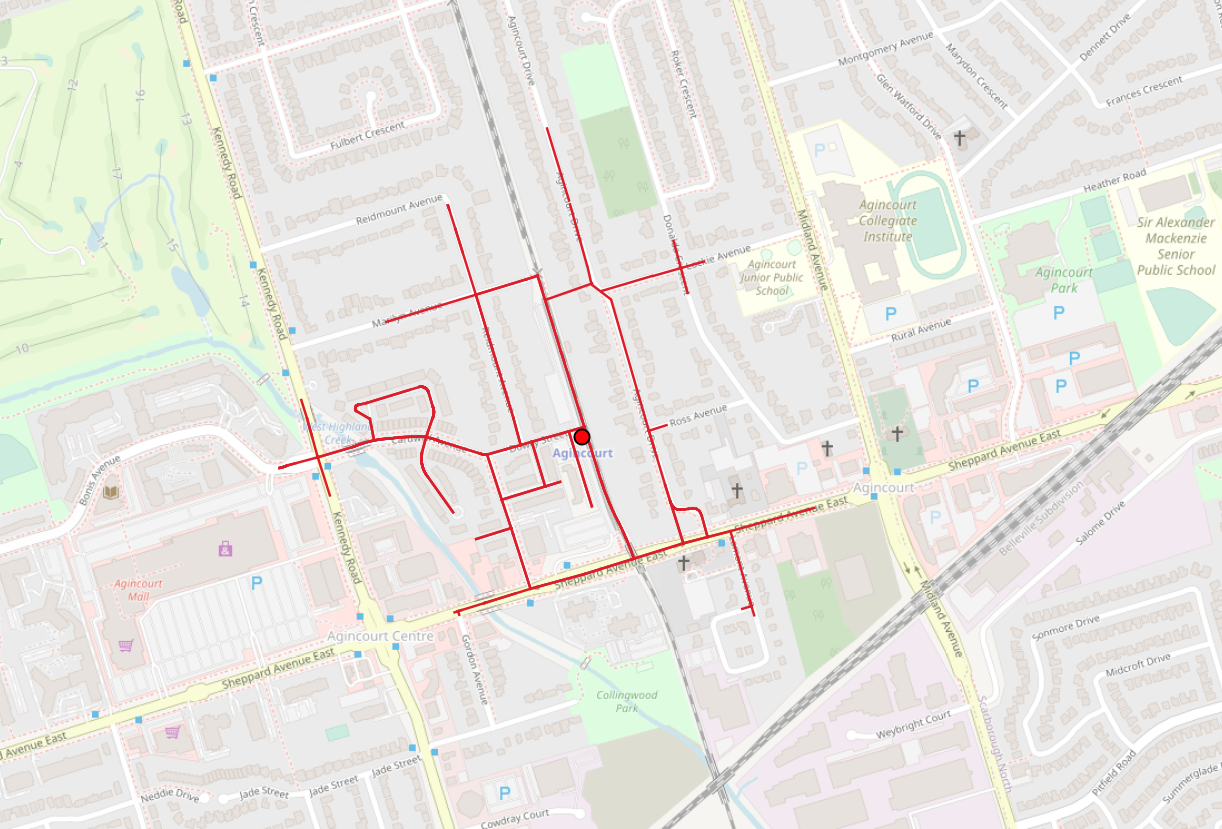
\includegraphics[width=1\linewidth]{images/agincourt.png}
			\end{figure}
			
		\end{column}
		
	\end{columns}
	
	
	
\end{frame}


\begin{frame}
	
	\textbf{Routes} - Stop Spacing, e.g. having "express" and "local" buses
	
	\begin{figure}
		\centering
		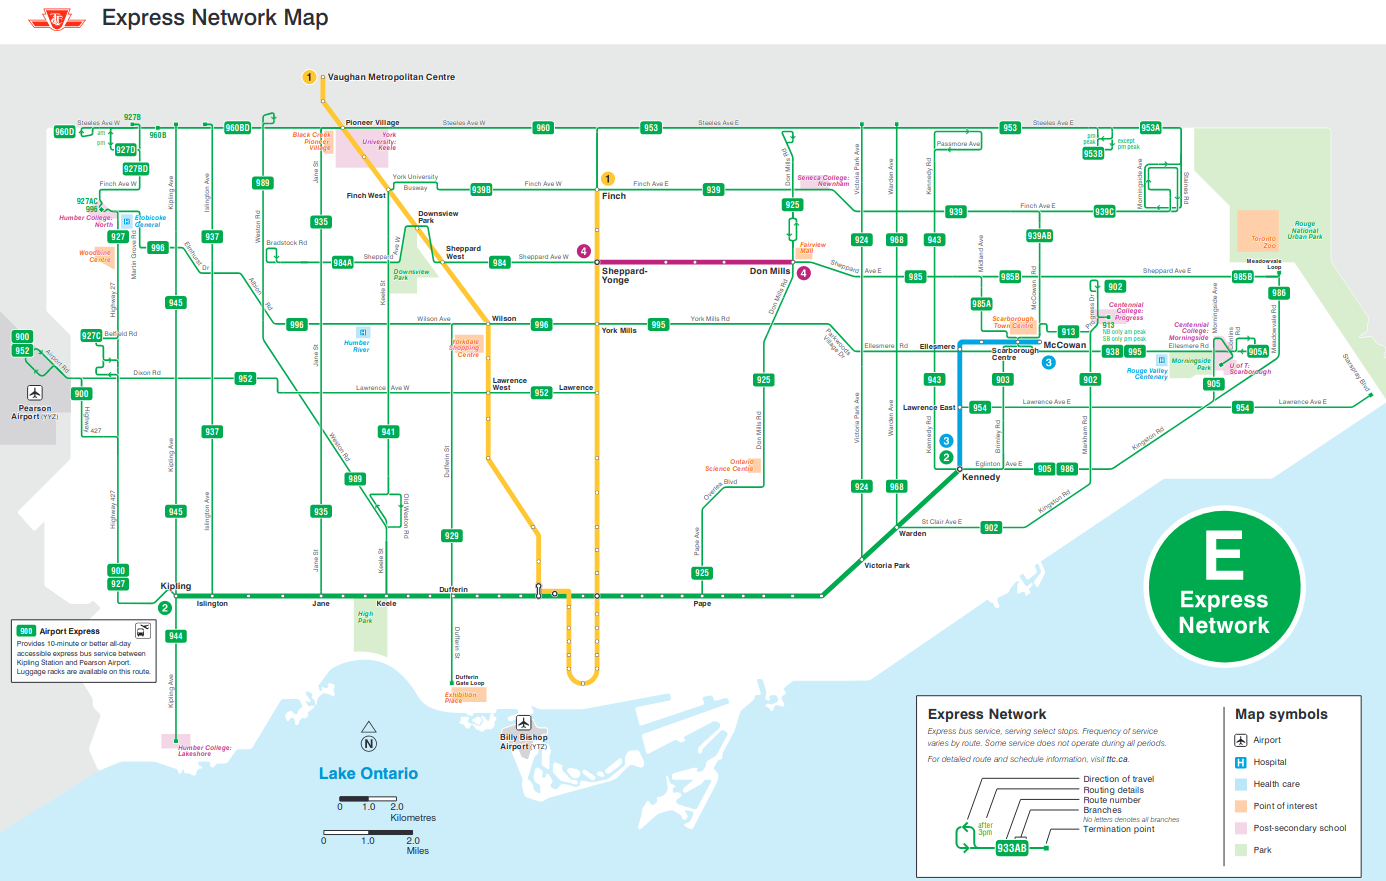
\includegraphics[width=0.9\linewidth]{images/ttc_express.png}
	\end{figure}
	
	
\end{frame}



\begin{frame}
	
	\textbf{Routes} - Reliability
	
	\vspace{2mm}
	
	Does the vehicle arrive on time?
	
	\vspace{2mm}
	

		\begin{figure}
			\centering
			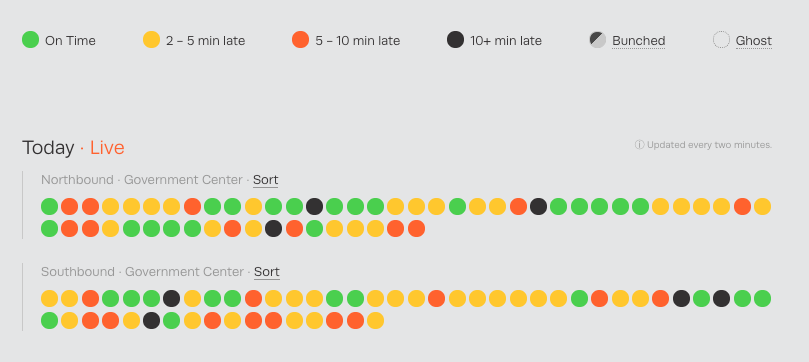
\includegraphics[width=1\linewidth]{images/transit-miami-screenshot.png}
		\end{figure}

	
\end{frame}


\begin{frame}
	
	\textbf{Routes} - Reliability
	
	\vspace{2mm}
	
	Expected travel times, e.g. along King Street before and after reducing traffic:
	
	\begin{figure}
		\centering
		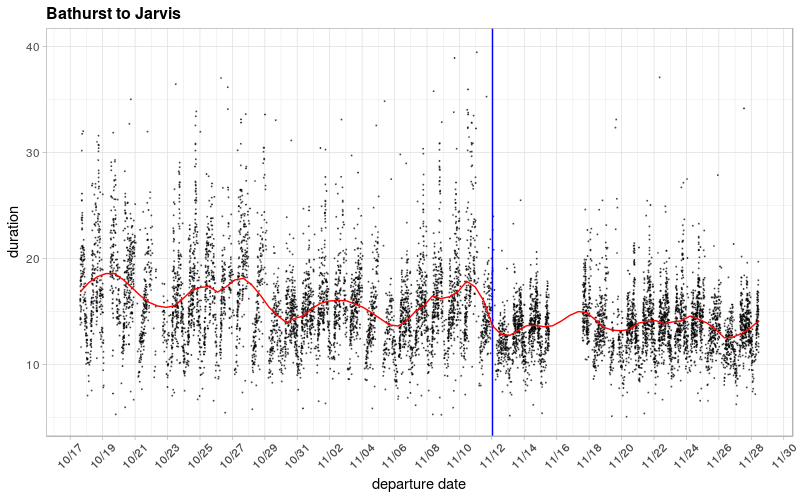
\includegraphics[width=0.8\linewidth]{images/king-street.png}
	\end{figure}
	
	
\end{frame}



\begin{frame}
	
	\textbf{Routes} - Reliability
	
	\vspace{2mm}
	
	What causes "bus bunching"?
	
	\begin{figure}
		\centering
		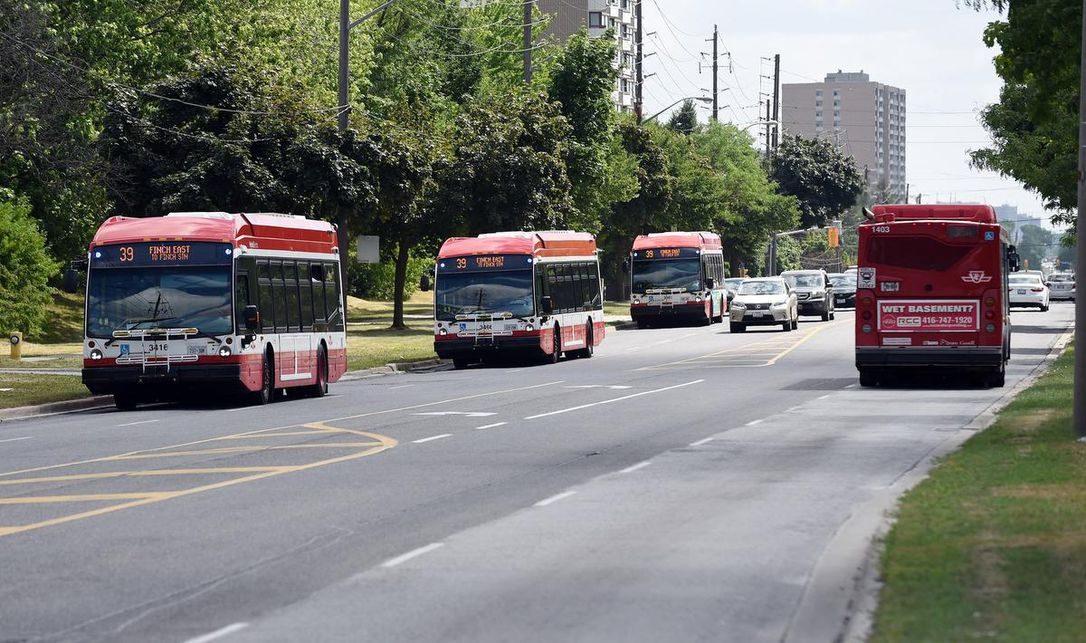
\includegraphics[width=0.8\linewidth]{images/finch39.jpg}
	\end{figure}
	
	
\end{frame}



\begin{frame}
	
	\textbf{Routes} - Reliability
	
	\vspace{2mm}
	
	What causes "bus bunching"?
	
	\begin{figure}
		\centering
		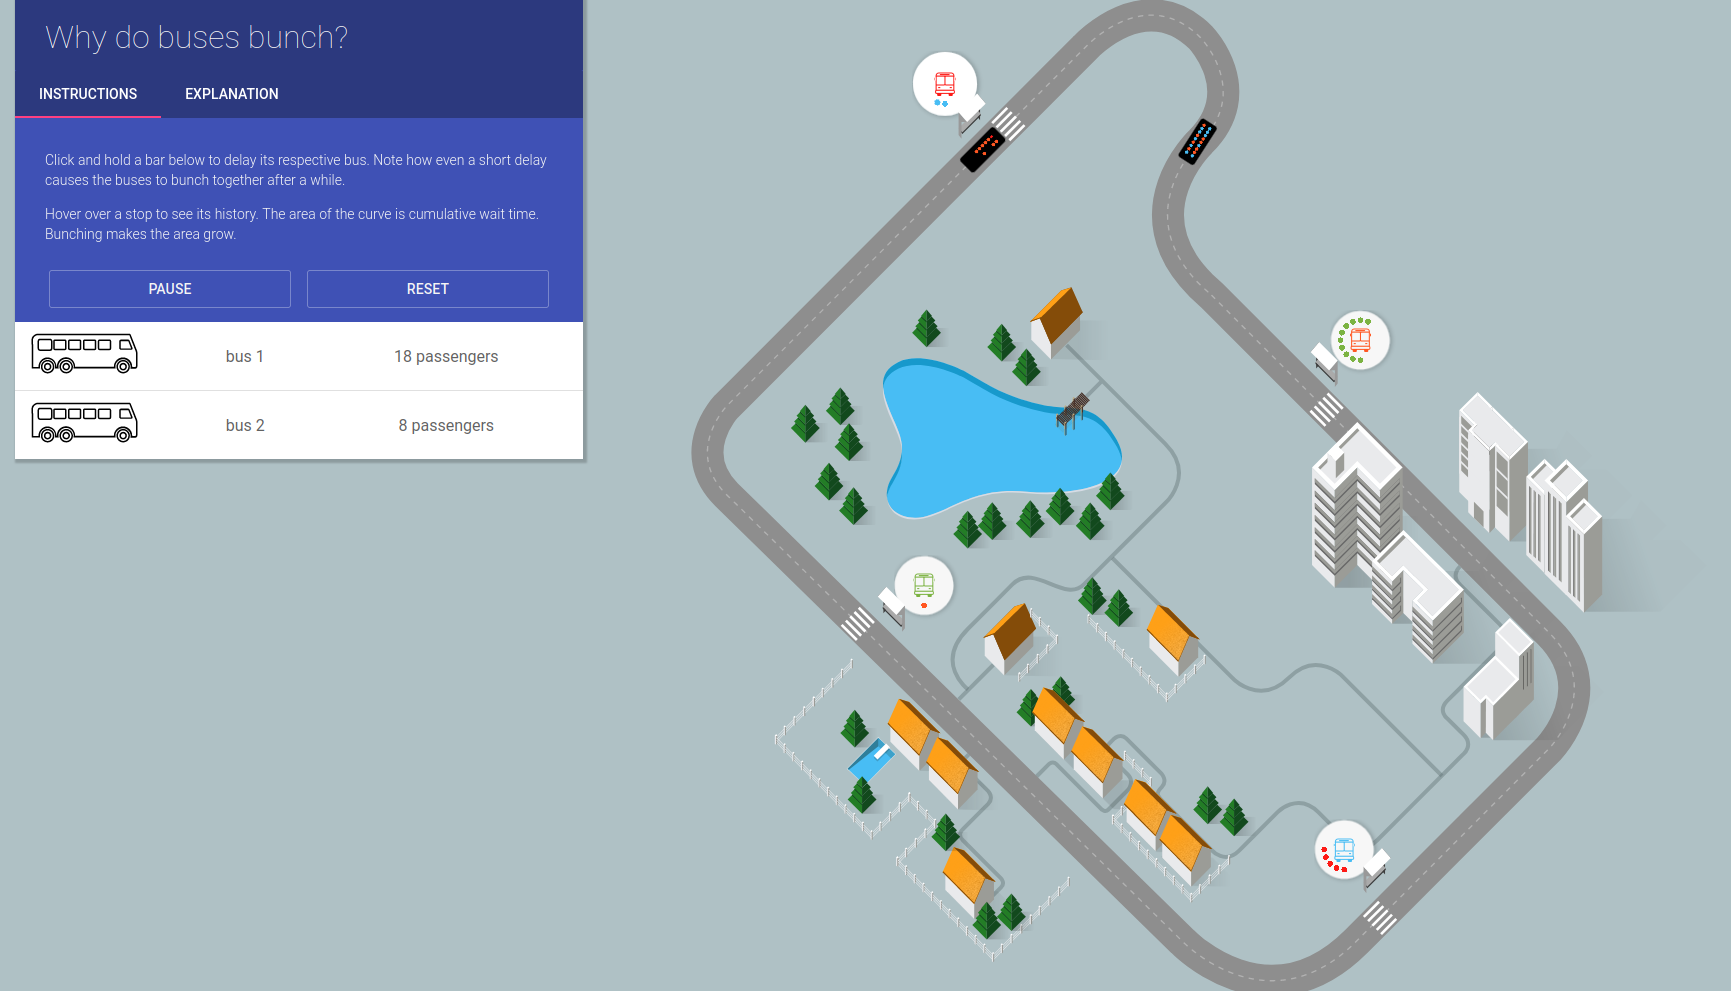
\includegraphics[width=0.8\linewidth]{images/bus-bunching.png}
	\end{figure}
	
	
	\tiny \url{https://setosa.io/bus/}
	
\end{frame}



\begin{frame}
	
	\textbf{Routes} - Unreliability affects wait times:
	
	\vspace{4mm}
	
	A simple formula:
	
	\[
	T_w = \frac{\sum_i S_i S_i / 2}{\sum_i S_i}
	\]
	
	$S_i$ = time between arrivals
	
	$S_i / 2$ = average wait time between each vehicle (assuming random departures)
	
	$T_w$ = total average wait time
	
	
	\begin{figure}
		\centering
		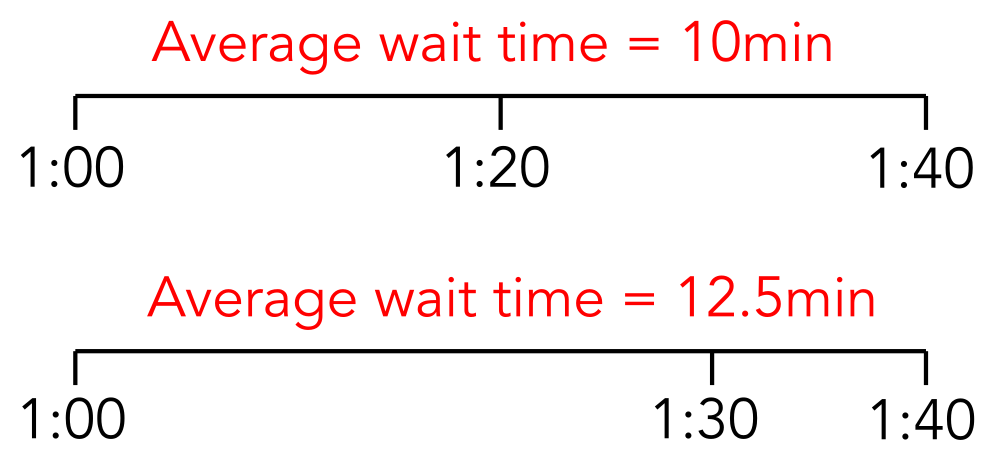
\includegraphics[width=0.6\linewidth]{images/wait_time.png}
	\end{figure}
	
	
\end{frame}





\begin{frame}
	
	\textbf{Fare Types}
	\begin{itemize}
		\item Flat fares (e.g. TTC)
		\item By distance (e.g. GO Transit)
		\item By zone
		\item Daily/weekly/monthly passes
		\item Discounts (e.g., child, students, senior, low-income)
		\item No fare
	\end{itemize}

	\textbf{Payment Technology}
	\begin{itemize}
		\item Cash
		\item Tokens/Tickets
		\item Card (ca be tap on only, or tap on and off)
	\end{itemize}
	
	
\end{frame}




\begin{frame}
	
	\textbf{Fares} - e.g. TTC Fares over time
	
	\begin{figure}
		\centering
		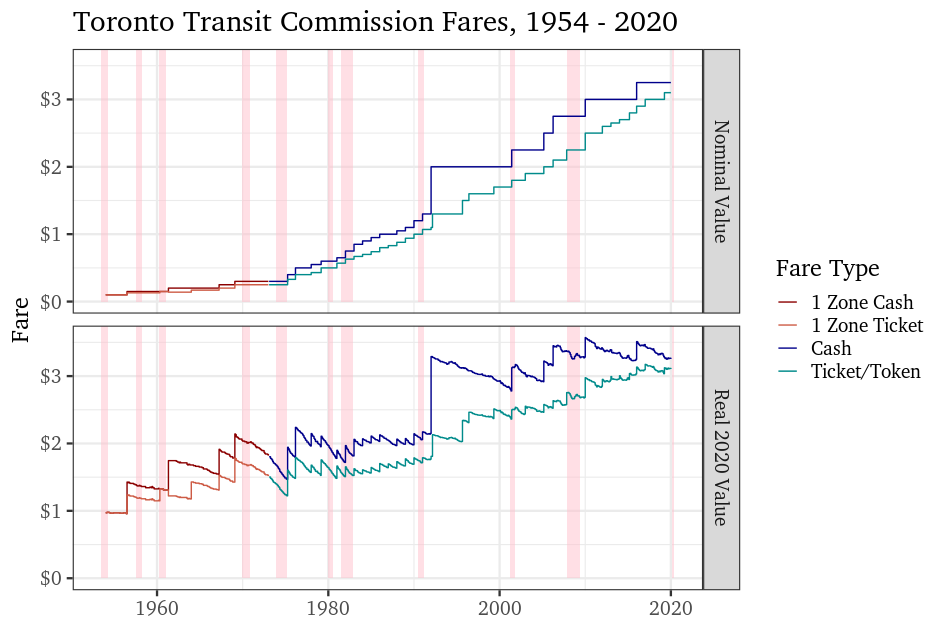
\includegraphics[width=0.8\linewidth]{images/ttc-fares.png}
	\end{figure}
	
	\tiny\url{https://github.com/Nate-Wessel/TTC-funding}
	
\end{frame}





\begin{frame}
	
	\textbf{Stops} - Local Stops
	
	\begin{figure}
		\centering
		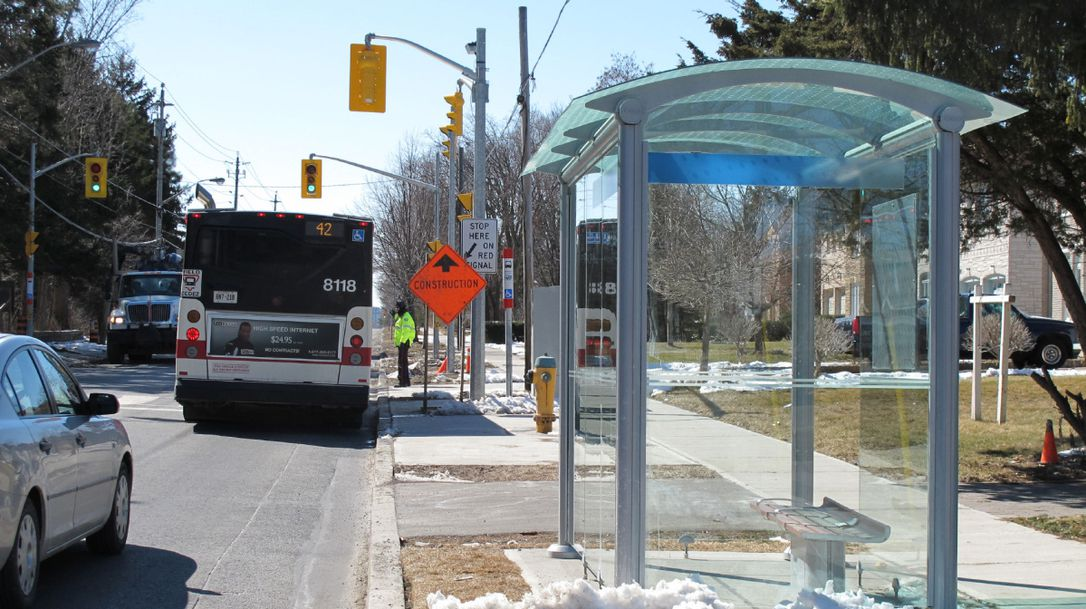
\includegraphics[width=0.8\linewidth]{images/bus_stop_ttc.jpeg}
	\end{figure}
	
\end{frame}




\begin{frame}
	
	\textbf{Stops} - Transferring
	
	\begin{figure}
		\centering
		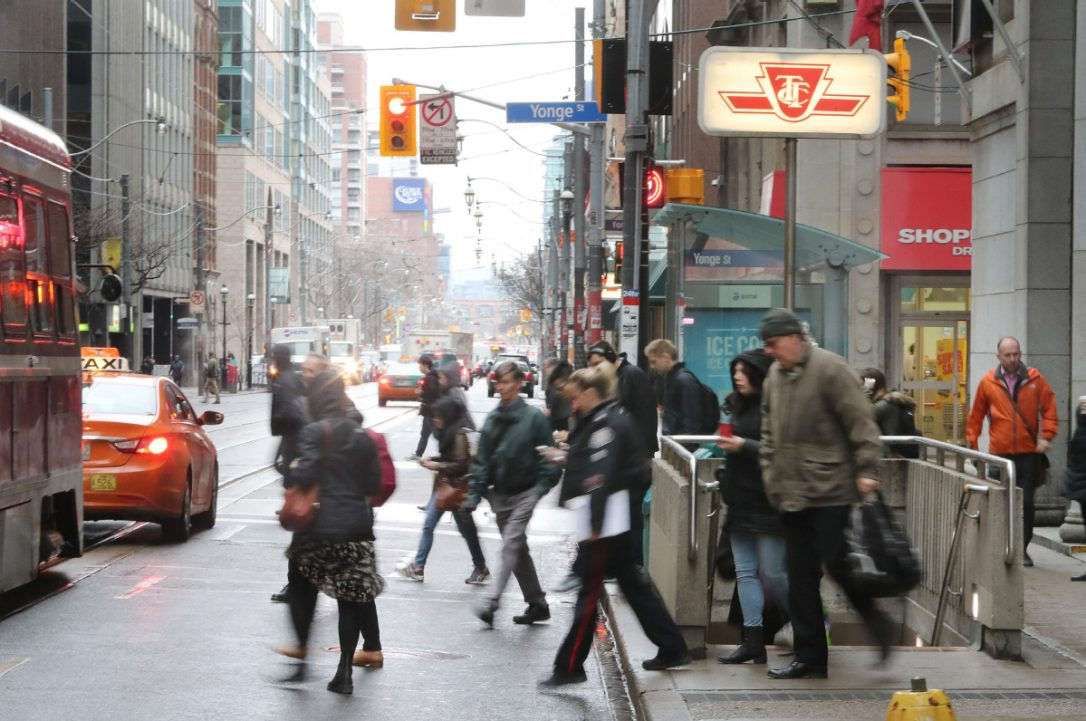
\includegraphics[width=0.8\linewidth]{images/ttc_transfer.jpg}
	\end{figure}
	
\end{frame}








\begin{frame}
	
	\textbf{Stops} - Major stations are key transferring locations
	
	\begin{figure}
		\centering
		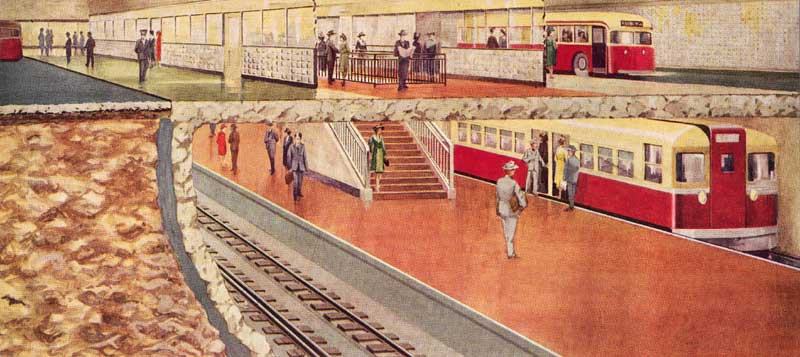
\includegraphics[width=0.98\linewidth]{images/eglinton_old_toronto.jpg}
	\end{figure}

	\tiny\url{https://www.toronto.ca/explore-enjoy/history-art-culture/online-exhibits/web-exhibits/web-exhibits-transportation/canadas-first-subway/canadas-first-subway-why-a-subway/}
	
\end{frame}



\begin{frame}
	
	\textbf{Stops} - Major stations can be iconic public spaces:
	
	\begin{figure}
		\centering
		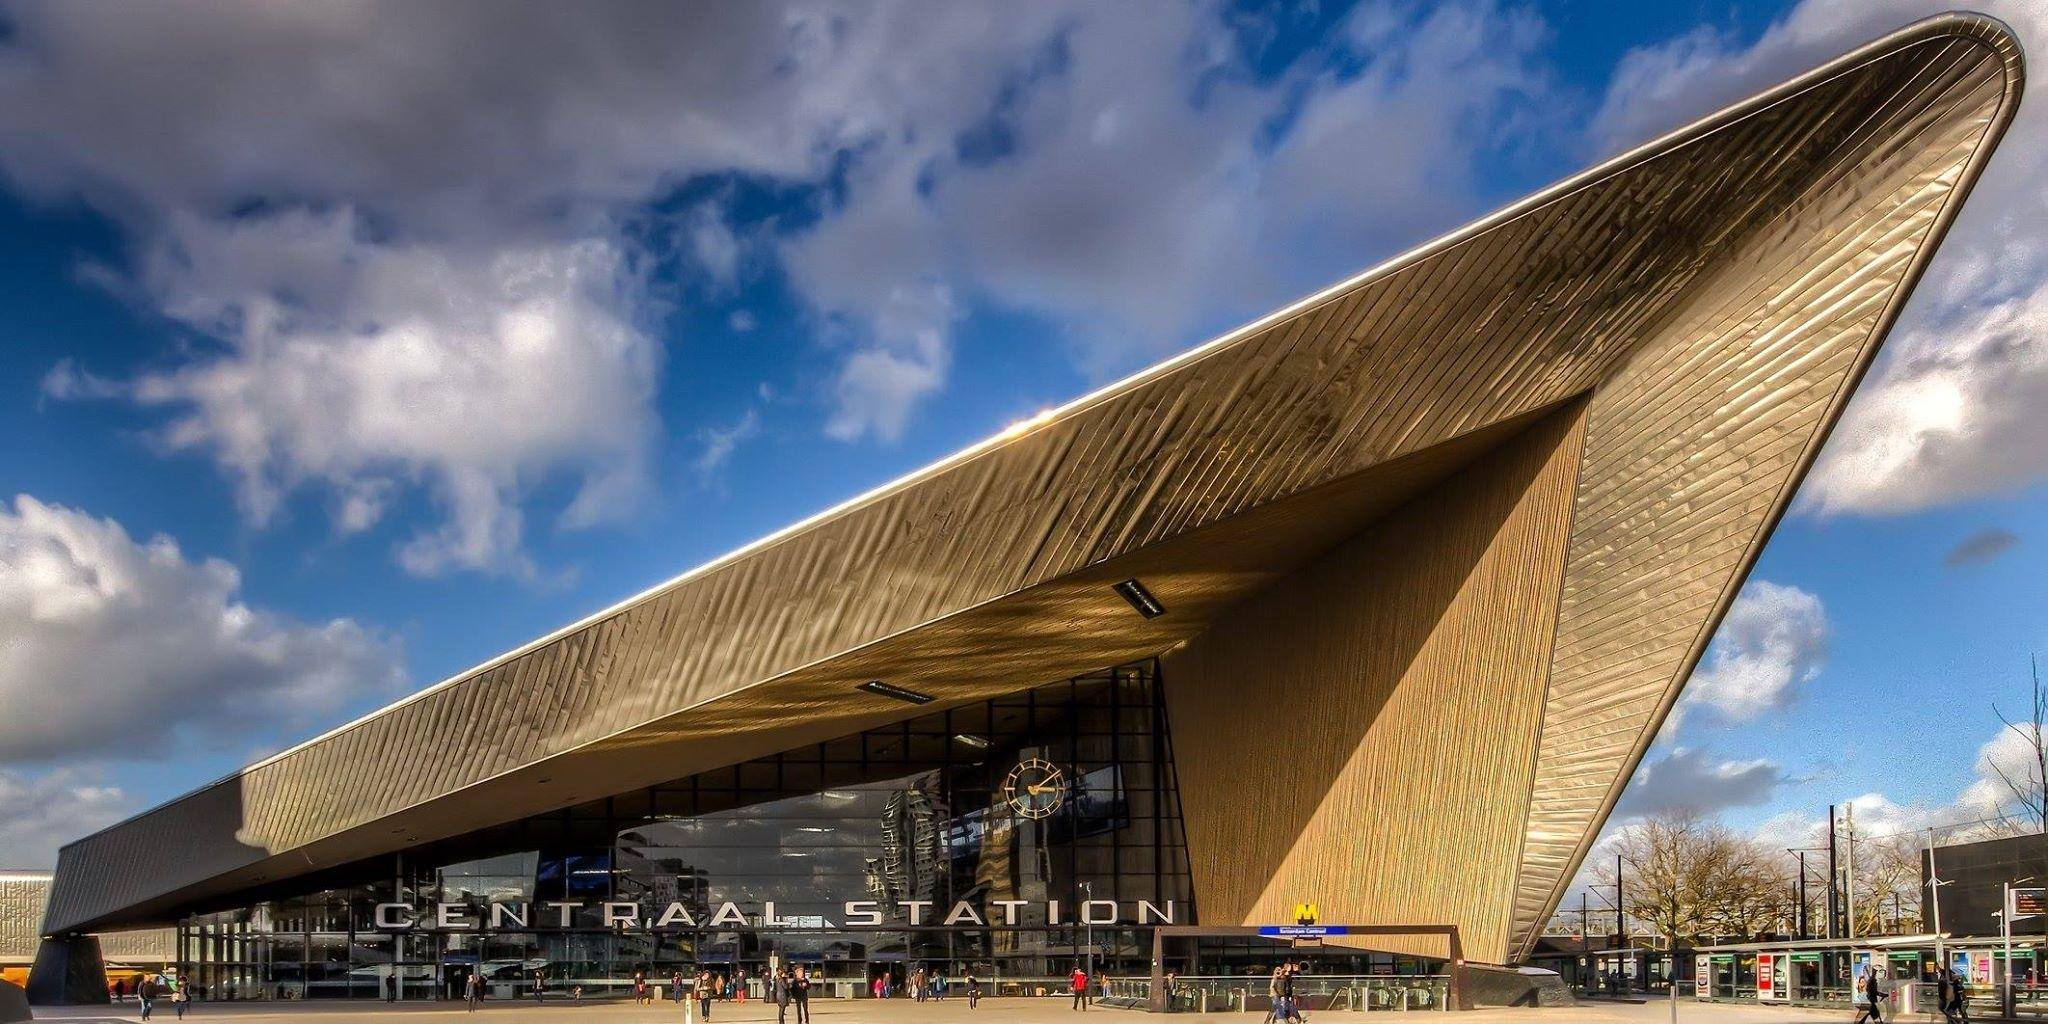
\includegraphics[width=0.98\linewidth]{images/rotterdam.jpg}
	\end{figure}

	\tiny\url{https://www.reddit.com/r/architecture/comments/20ceny/the_new_rotterdam_central_train_station_opened/}
	
\end{frame}




\begin{frame}
	
	



	\begin{columns}
		\begin{column}{0.5\textwidth}
			\textbf{Stops} - Access Mode
			
			\vspace{2mm}
			
			e.g. in the GTHA: 
			
			\begin{itemize}
				\item 91.8\% by walking
				\item 7.4\% by car
				\item 0.6\% by other mode (mostly bike)
			\end{itemize}
			
			
		\end{column}
		
		\begin{column}{0.5\textwidth}

			\begin{figure}
				\centering
				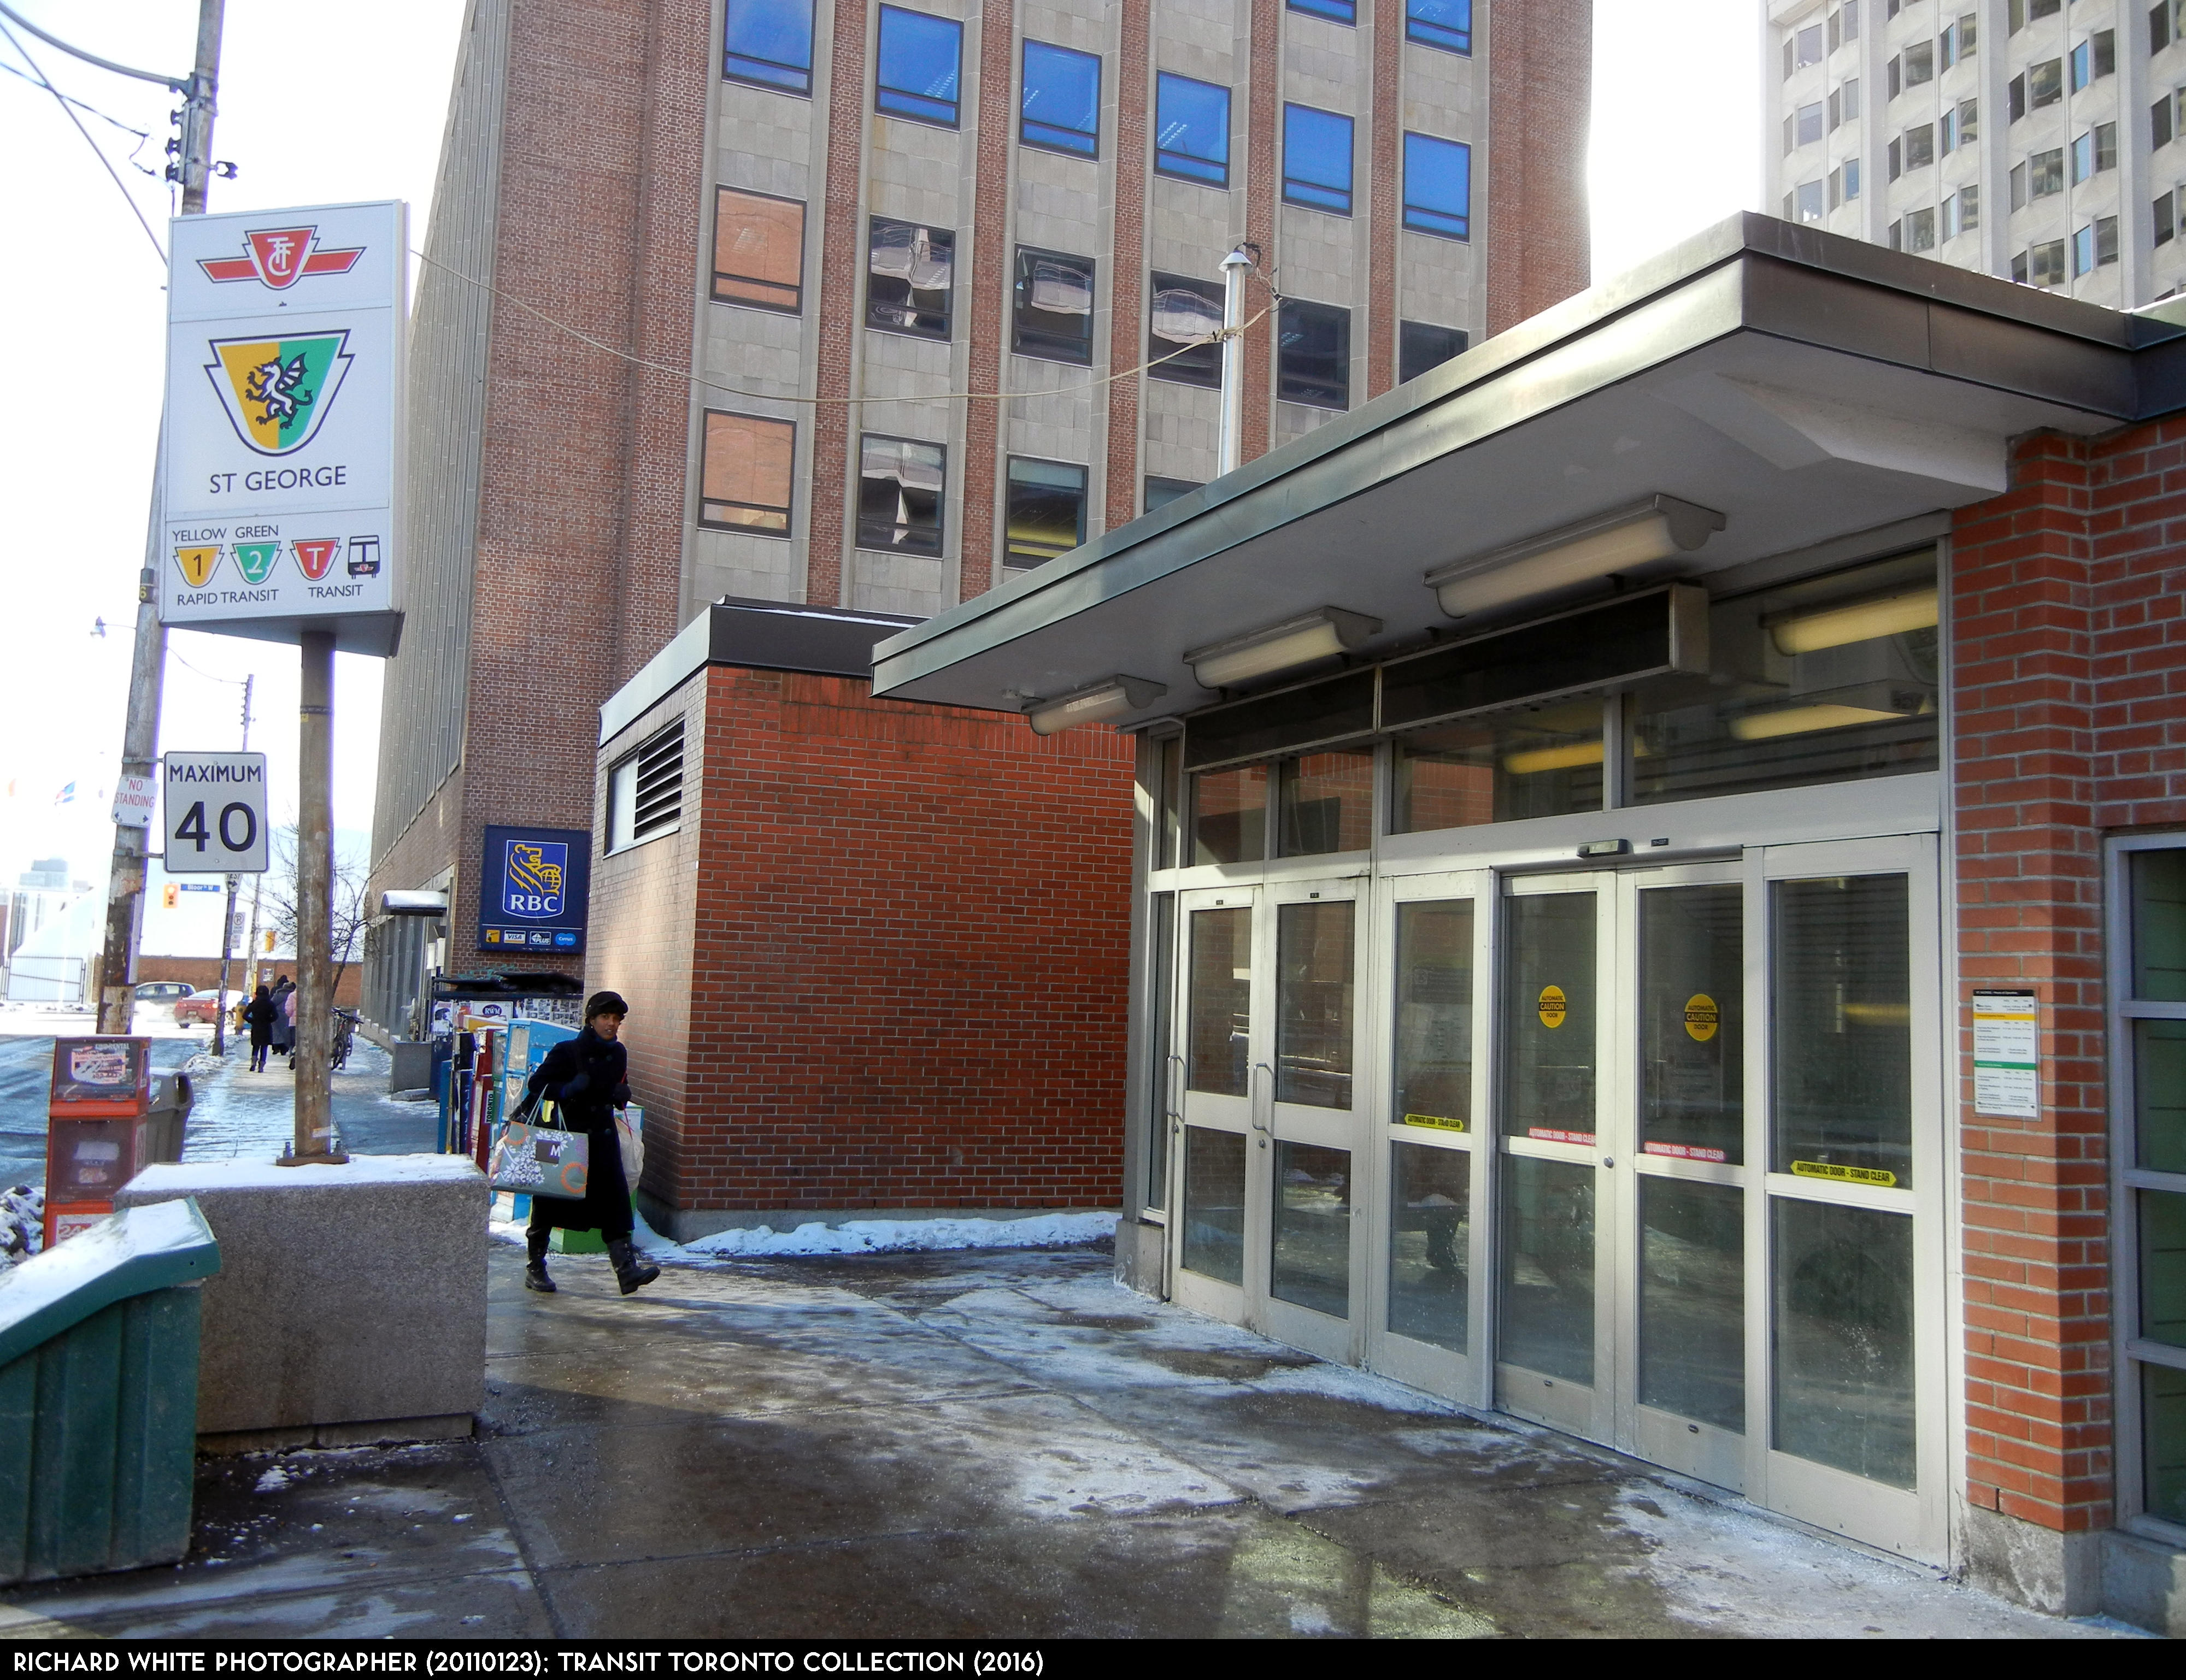
\includegraphics[width=1\linewidth]{images/st-george.jpg}
			\end{figure}
			
		\end{column}
		
	\end{columns}
		
\end{frame}



\begin{frame}
	
	\textbf{Stops} - Land-Use Around Stops
	
	\vspace{2mm}
	
	Whitby GO Station:
	\begin{figure}
		\centering
		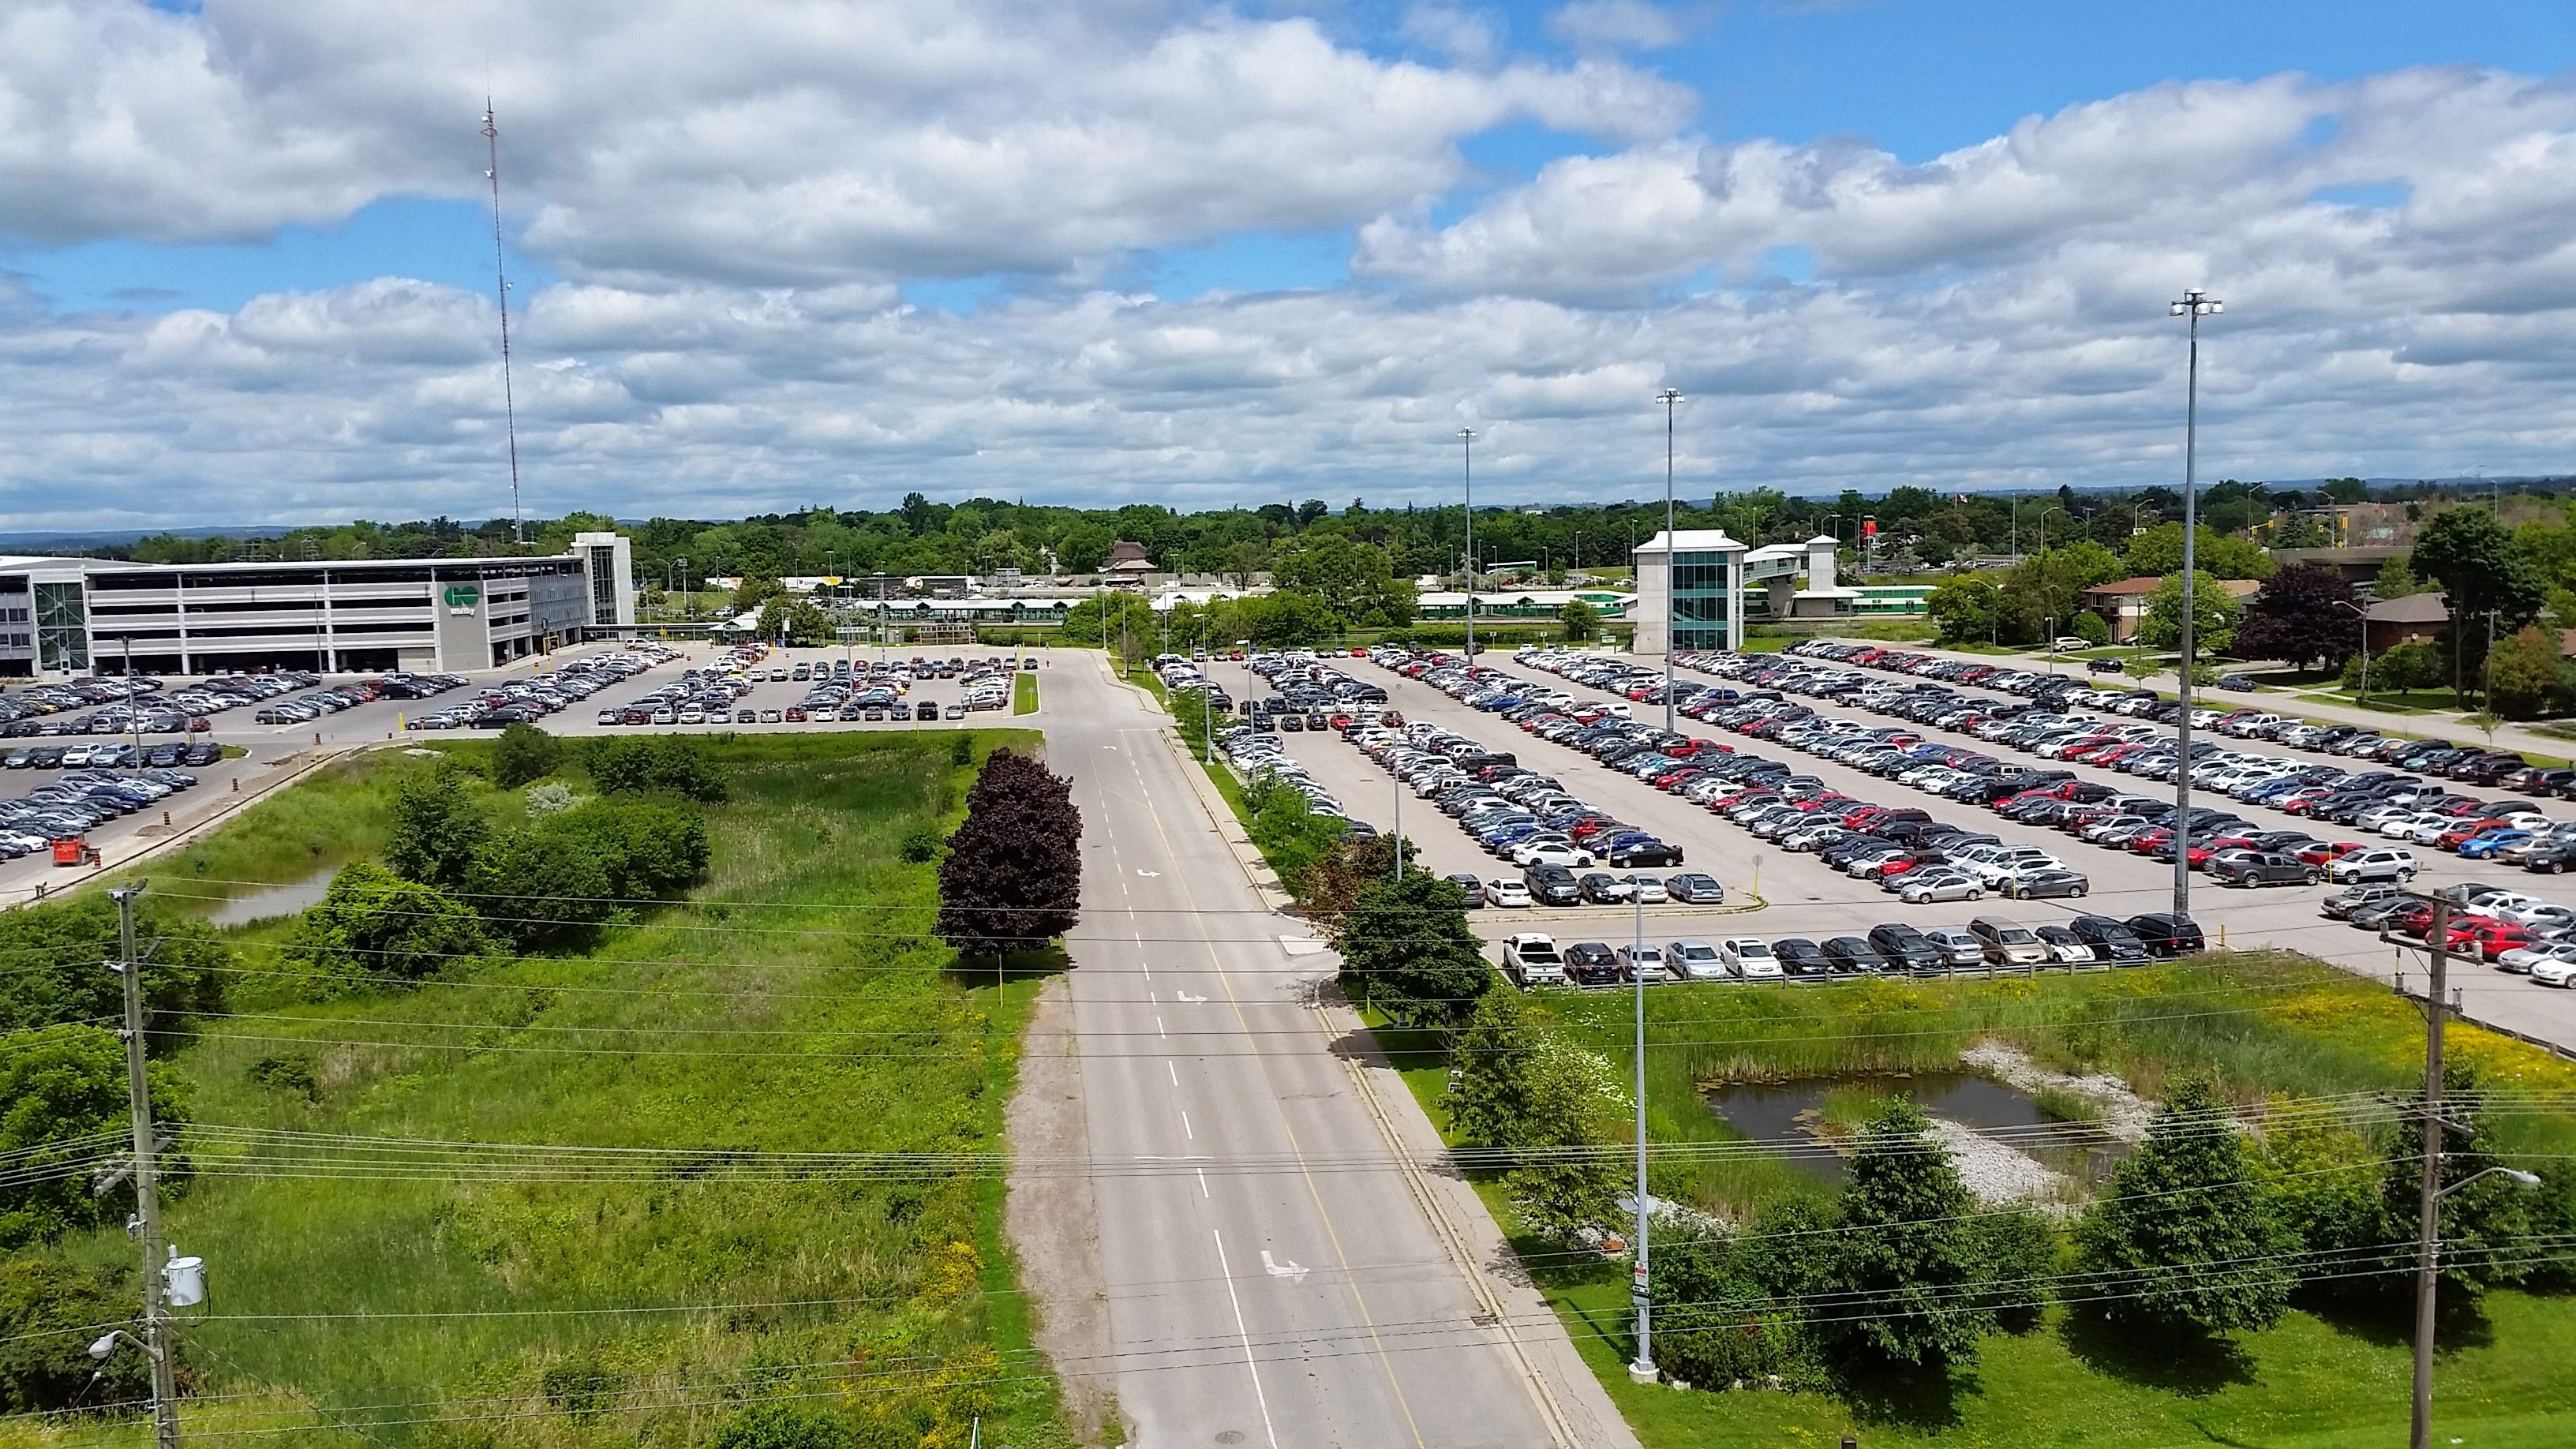
\includegraphics[width=0.98\linewidth]{images/whitby.jpg}
	\end{figure}
	
\end{frame}




\begin{frame}
	
	\textbf{Transit Oriented Development}
	\begin{itemize}
		\item Focusing urban development near major public transit hubs
		\item Often includes a mix of residential, retail, and commercial buildings
		\item Goals include increasing transit ridership, local active travel, and reducing sprawl
	\end{itemize}

	\begin{figure}
		\centering
		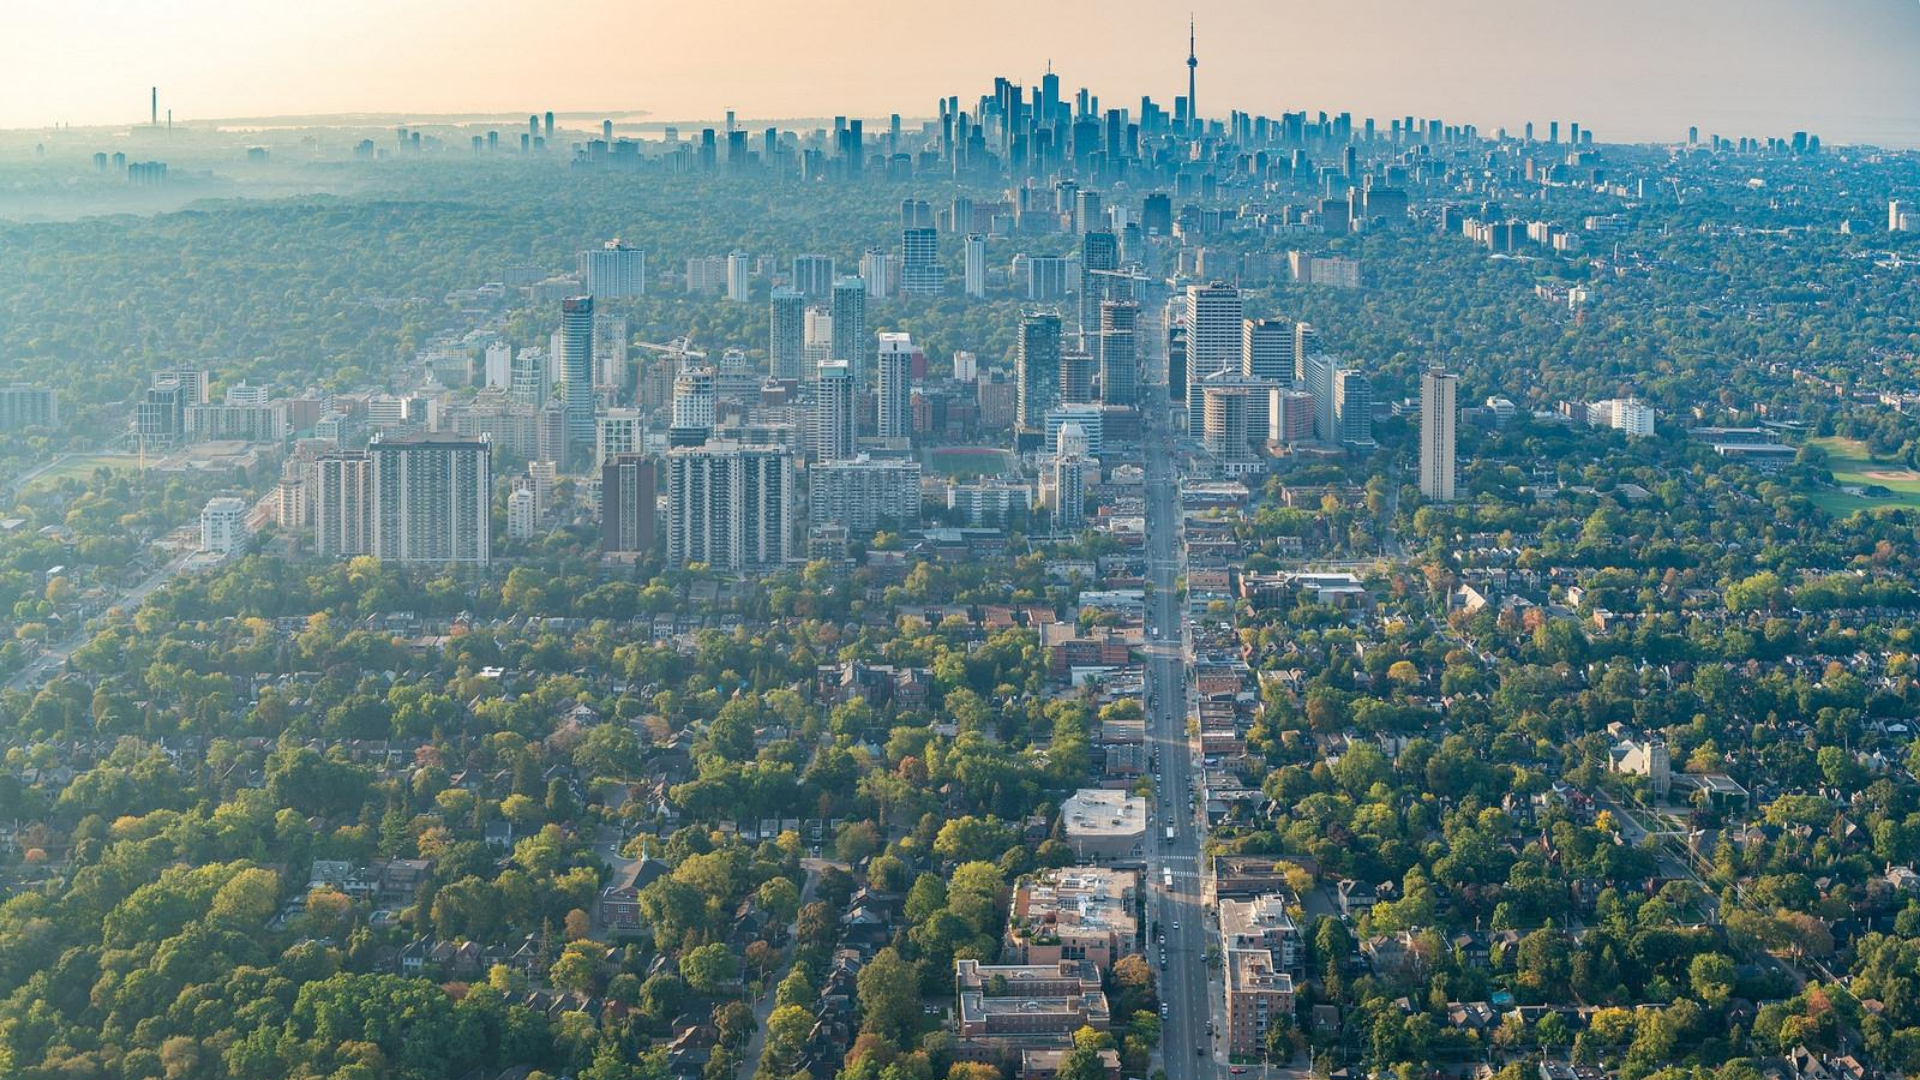
\includegraphics[width=0.78\linewidth]{images/i3.png}
	\end{figure}
		
\end{frame}




\begin{frame}
	
	\textbf{Transit Oriented Development}
	
	e.g. Marine Drive Station in Vancouver, when built in 2009 and in 2018
	
	\begin{columns}
		\begin{column}{0.5\textwidth}
			
			
			\begin{figure}
				\centering
				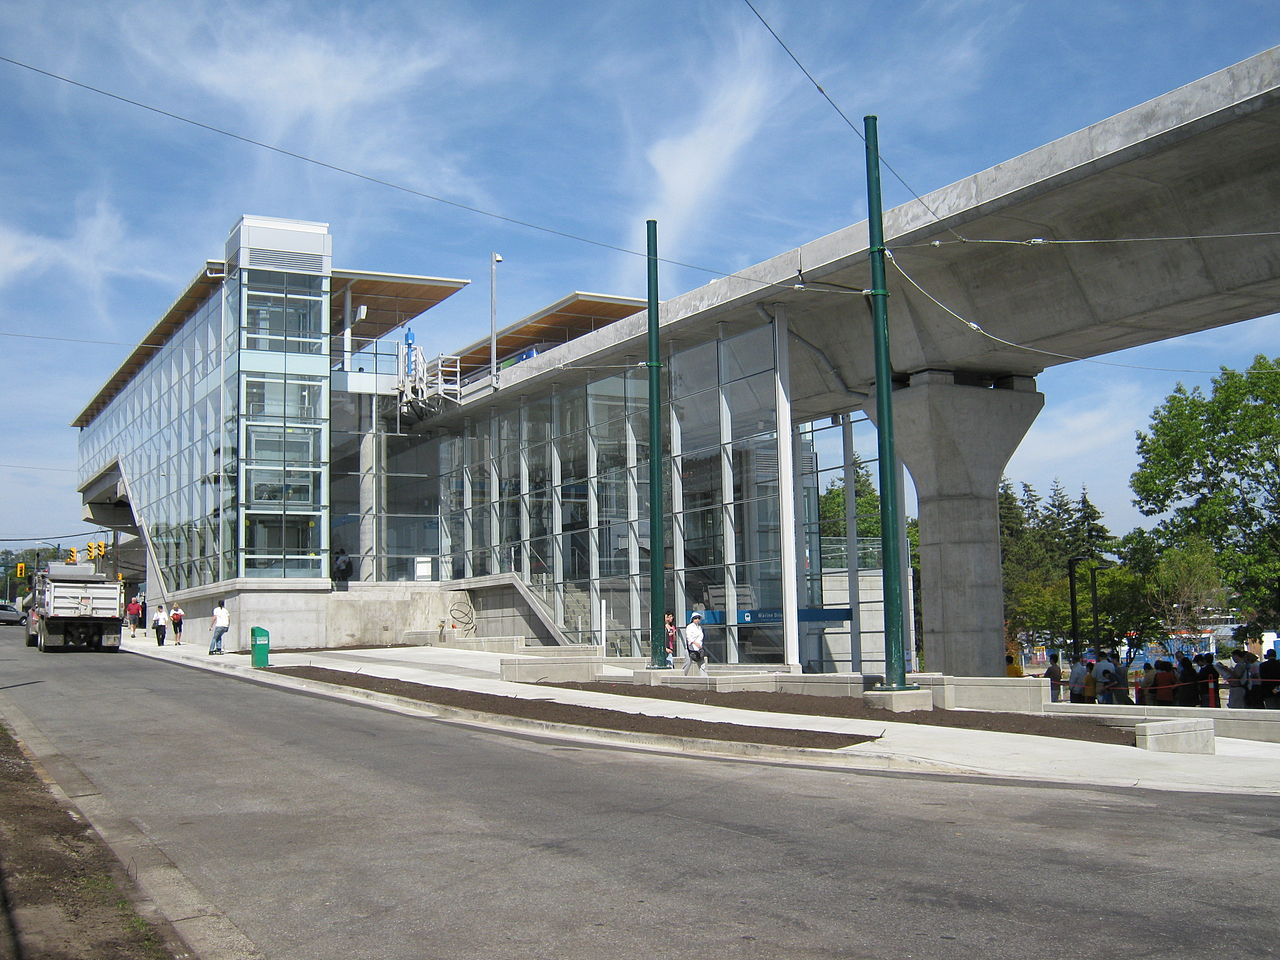
\includegraphics[width=1\linewidth]{images/marine_2009.jpg}
			\end{figure}
			
			
		\end{column}
		
		\begin{column}{0.5\textwidth}
			
			\begin{figure}
				\centering
			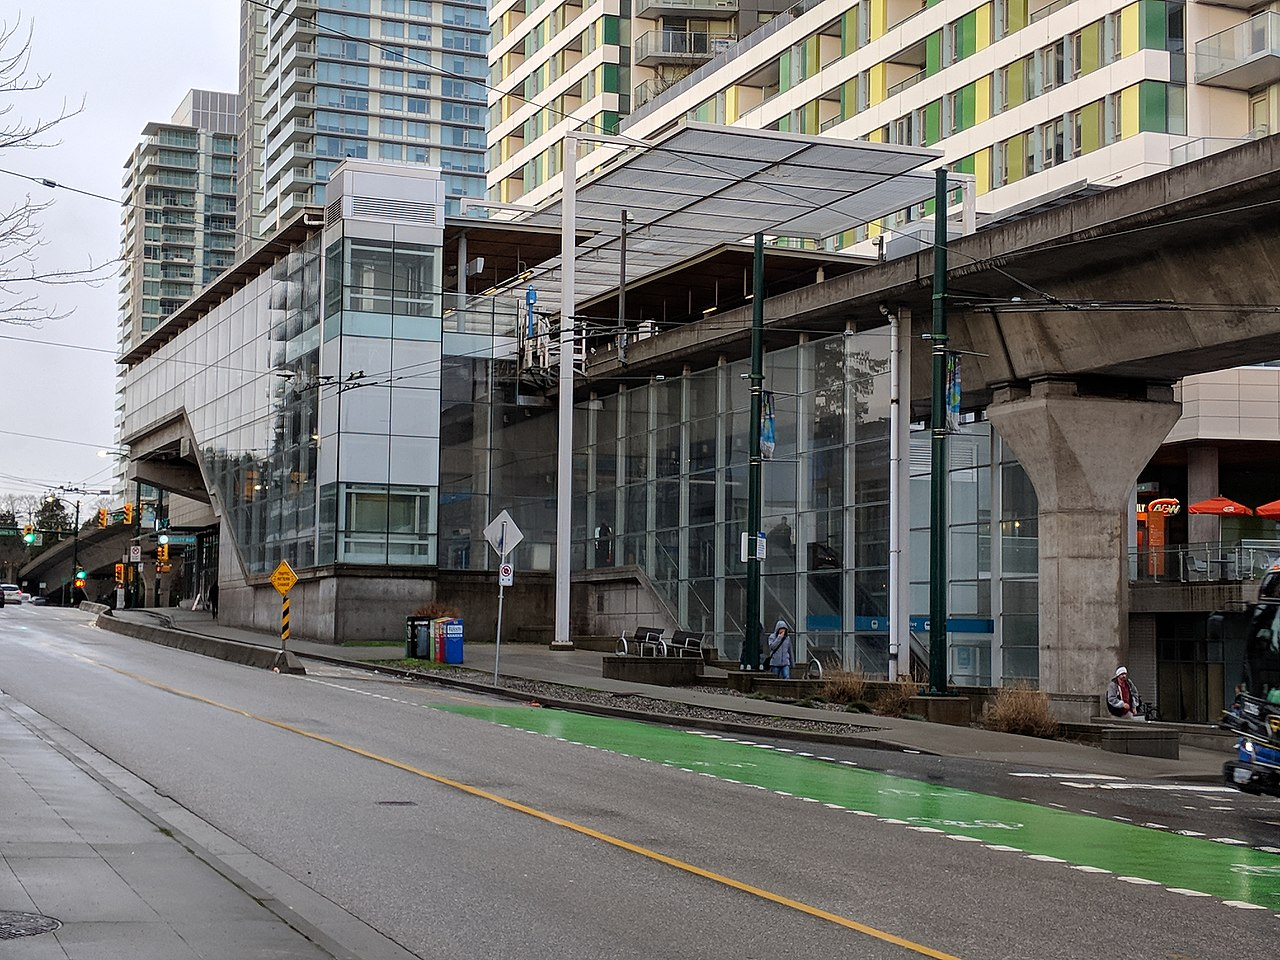
\includegraphics[width=1\linewidth]{images/marine_2018.jpg}
			\end{figure}
			
		\end{column}
		
	\end{columns}

	\vspace{2mm}

	\tiny\url{https://www.google.ca/maps/@49.2081409,-123.1191561,497a,35y,50.44h,34.64t/data=!3m1!1e3}
	
	\tiny\url{https://en.wikipedia.org/wiki/Transit-oriented_development}
	
\end{frame}




\begin{frame}
	
	\textbf{Transit Oriented Development}
	
	\vspace{2mm}
	
	Key(s) to Building Transit-Oriented Development?
	
	\begin{figure}
		\centering
		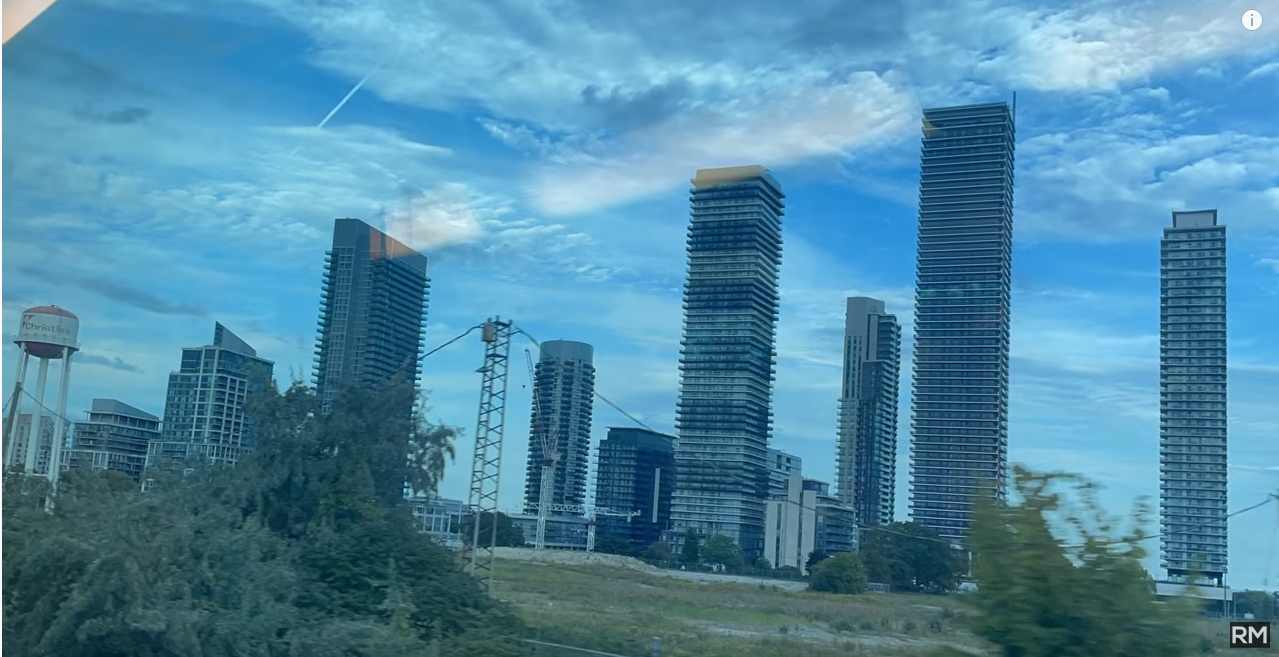
\includegraphics[width=0.7\linewidth]{images/humber_bay.png}
	\end{figure}
		
	
	\tiny 
	RMTransit
	 Video \url{https://www.youtube.com/watch?v=5HSI_PZBsPc}
	
	\vspace{2mm}
	
	\tiny More about Humber Bay Shores plan \url{https://urbantoronto.ca/database/projects/2150-lake-shore}
	
\end{frame}



\begin{frame}
	
	\textbf{Public Transit Planning}
	
	- about improving public transit, with both big and small ideas

		\begin{figure}
			\centering
			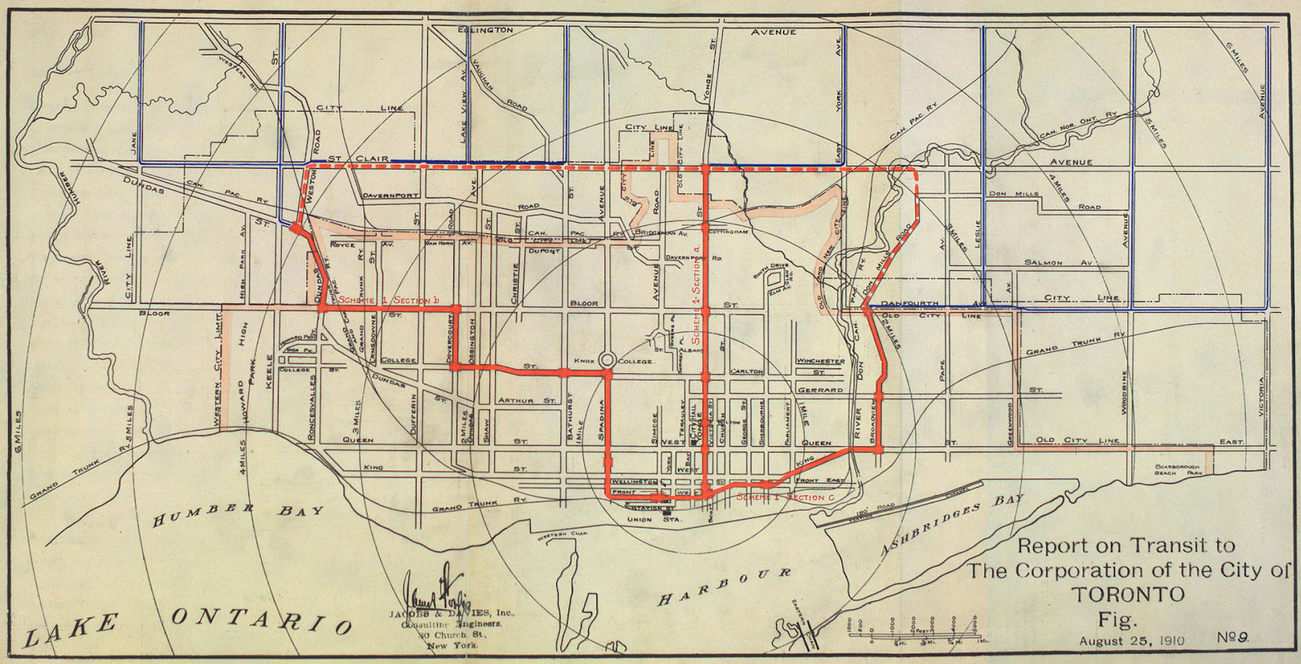
\includegraphics[width=0.9\linewidth]{images/toronto_plan_1910.png}
		\end{figure}
	
\end{frame}



\begin{frame}
	
	\textbf{Public Transit Planning}
	
	
	\begin{figure}
		\centering
		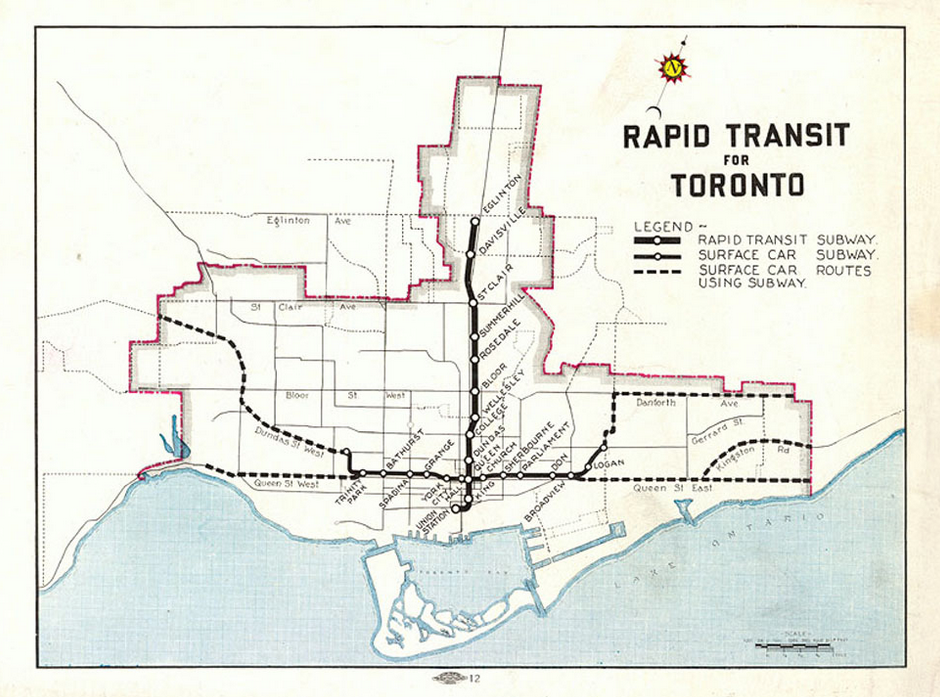
\includegraphics[width=0.8\linewidth]{images/toronto_plan_1945.png}
	\end{figure}
		
\end{frame}



\begin{frame}
	
	\textbf{Public Transit Planning}

	
	\begin{figure}
		\centering
		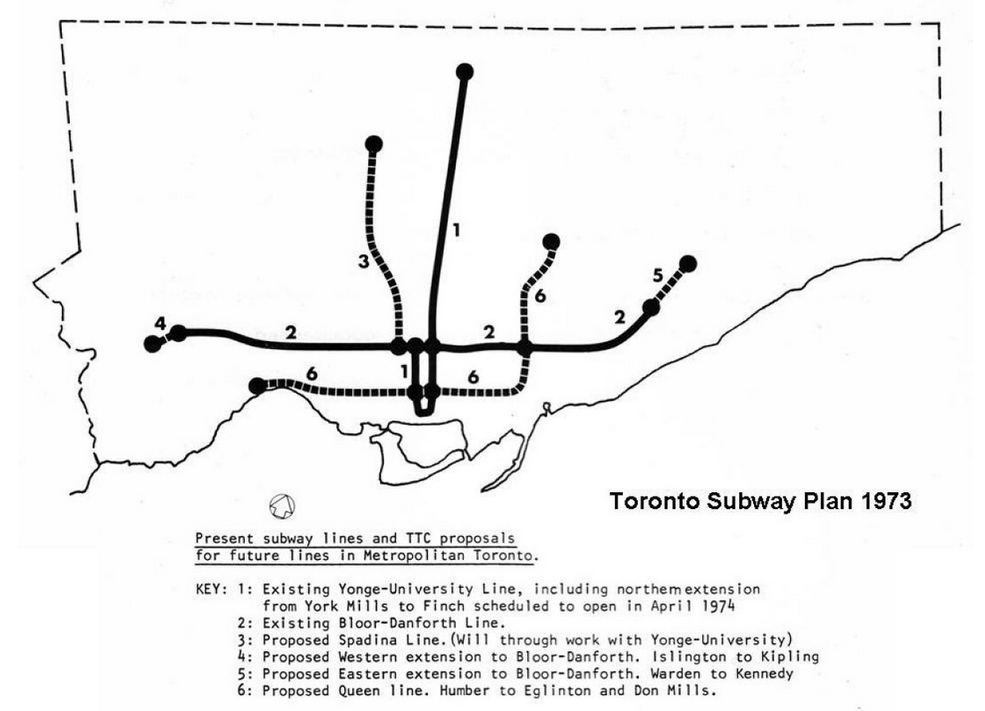
\includegraphics[width=0.8\linewidth]{images/toronto_plan_1973.png}
	\end{figure}
	
	
\end{frame}



\begin{frame}
	
	\textbf{Public Transit Planning}
	
	
	
	\begin{figure}
		\centering
		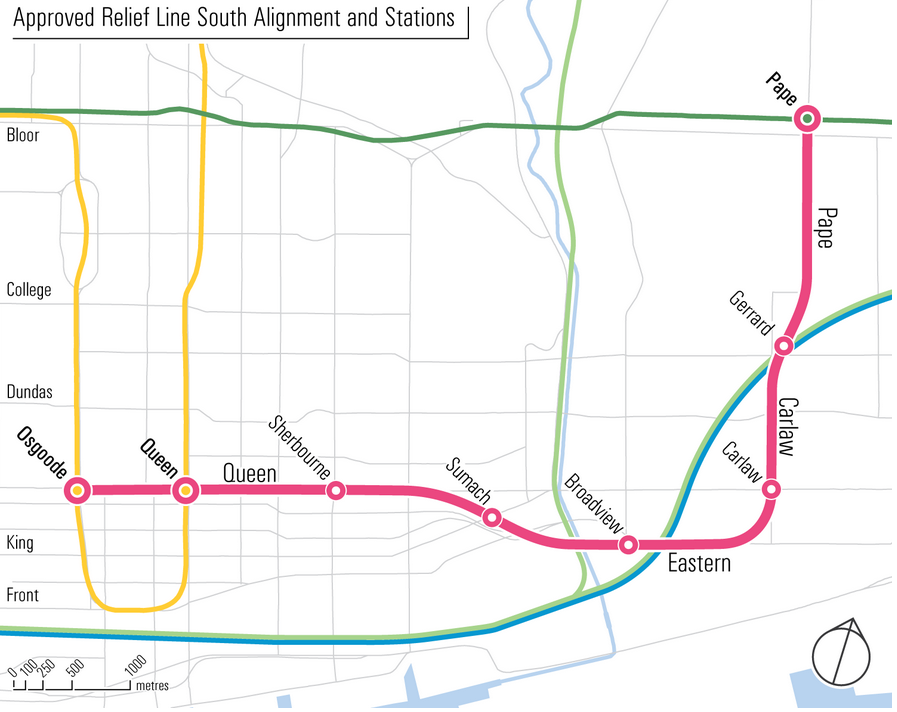
\includegraphics[width=0.8\linewidth]{images/toronto_plan_2019.png}
	\end{figure}
	
	
\end{frame}


\begin{frame}
	
	\textbf{Public Transit Planning}
	
	
	
	\begin{figure}
		\centering
		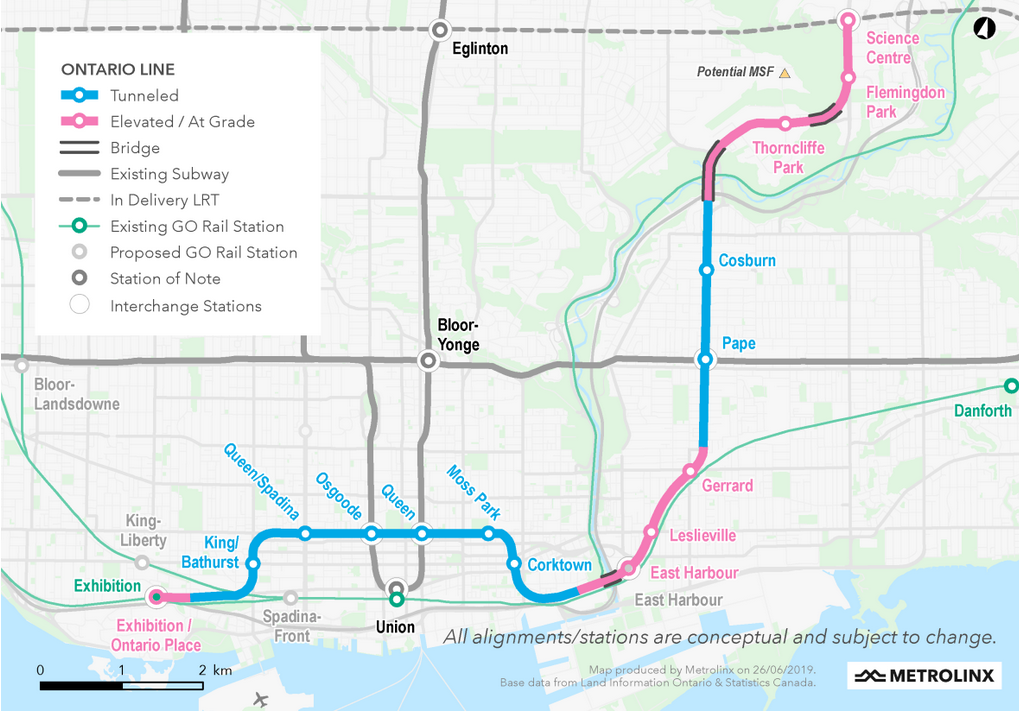
\includegraphics[width=0.8\linewidth]{images/mx_plan_2019.png}
	\end{figure}
	
	
\end{frame}






\begin{frame}
	
	\textbf{Public Transit Planning}
	
	
	
	\begin{figure}
		\centering
		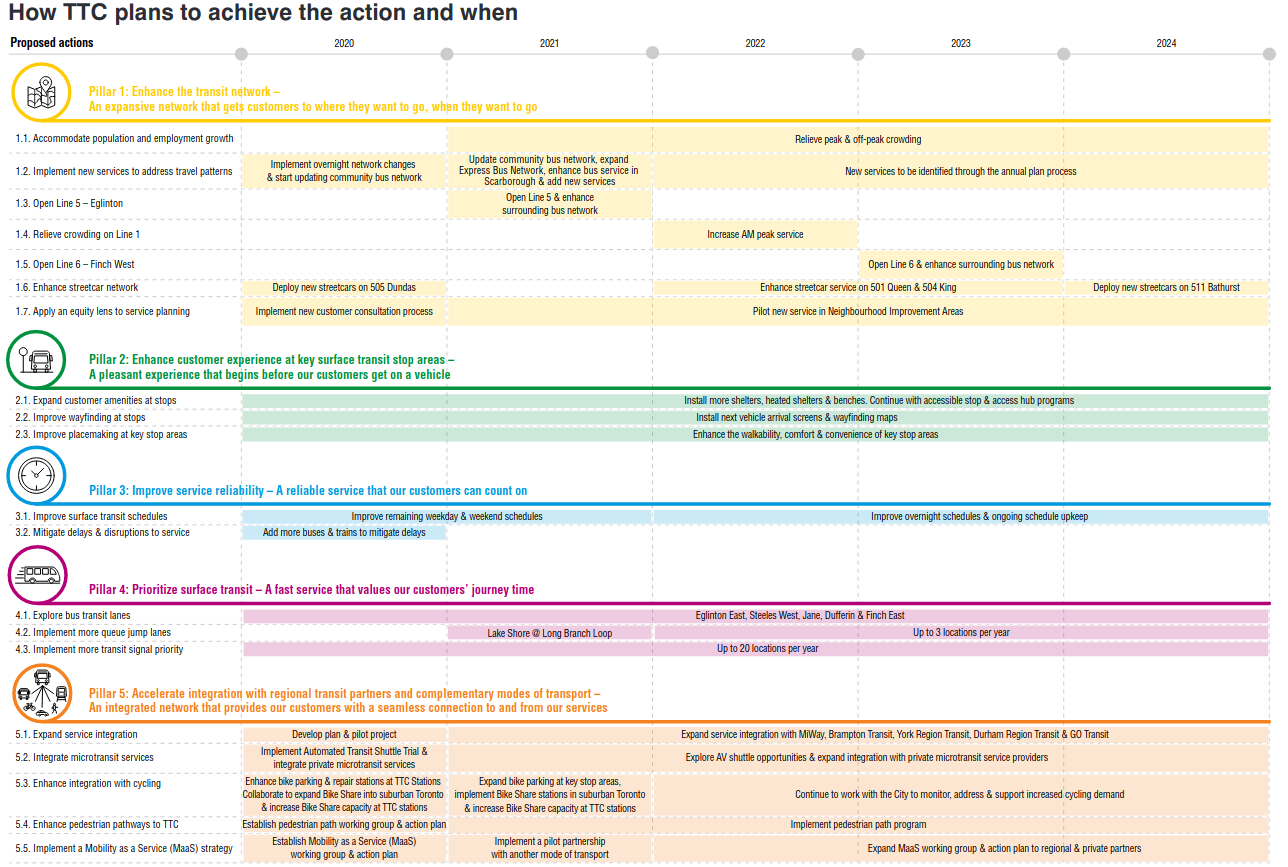
\includegraphics[width=0.8\linewidth]{images/ttc-5-year.png}
	\end{figure}
	
	\tiny\url{https://www.ttc.ca/about-the-ttc/projects-and-plans/5-Year-Service-Plan-and-10-Year-Outlook}
	
\end{frame}


% Transit Planning
% about future improvements, or new lines



\begin{frame}
	
	Next week (Feb 7)
	
	\begin{itemize}
		\item Transportation and land-use
		\item Network analysis \& GIS
		\item Land-use data
		\item Measuring accessibility
	\end{itemize}

	Following week (Feb 14)
	
	\begin{itemize}
		\item Travel surveys
		\item Other transportation-related data
		\item Maps for navigation
		\item Chat about the assignment
	\end{itemize}
	
\end{frame}








\end{document}